% Opcje klasy 'iithesis' opisane sa w komentarzach w pliku klasy. Za ich pomoca
% ustawia sie przede wszystkim jezyk oraz rodzaj (lic/inz/mgr) pracy.
\documentclass[shortabstract, mgr, english]{iithesis}

\usepackage[utf8]{inputenc}

%%%%% DANE DO STRONY TYTUŁOWEJ
% Niezaleznie od jezyka pracy wybranego w opcjach klasy, tytul i streszczenie
% pracy nalezy podac zarowno w jezyku polskim, jak i angielskim.
% Pamietaj o madrym (zgodnym z logicznym rozbiorem zdania oraz estetyka) recznym
% zlamaniu wierszy w temacie pracy, zwlaszcza tego w jezyku pracy. Uzyj do tego
% polecenia \fmlinebreak.
\polishtitle    {Funkcje normalizujące dla typów ilorazowych w Coqu}
\englishtitle   {Normalization functions \fmlinebreak for quotient types in Coq}
\polishabstract {\ldots}
\englishabstract{\ldots}
% w pracach wielu autorow nazwiska mozna oddzielic poleceniem \and
\author         {Marek Bauer}
% w przypadku kilku promotorow, lub koniecznosci podania ich afiliacji, linie
% w ponizszym poleceniu mozna zlamac poleceniem \fmlinebreak
\advisor        {dr Małgorzata Biernacka}
%\date          {}                     % Data zlozenia pracy
% Dane do oswiadczenia o autorskim wykonaniu
%\transcriptnum {}                     % Numer indeksu
%\advisorgen    {dr. Jana Kowalskiego} % Nazwisko promotora w dopelniaczu
%%%%%

%%%%% WLASNE DODATKOWE PAKIETY
\usepackage{amsfonts} 
\usepackage{stmaryrd}
\usepackage{minted}
\usepackage{polski}
\usepackage{graphicx}
\usepackage{MnSymbol}
\usepackage{tikz}
\usepackage{tikz-qtree}
\usepackage{enumitem}

\graphicspath{ {./img/} }
\usemintedstyle{tango}
\usetikzlibrary {arrows.meta}
\usepackage[framemethod=TikZ]{mdframed}

%%%%% WŁASNE DEFINICJE I POLECENIA
\definecolor{CoqIDE}{RGB}{255,248,220}
\definecolor{darkYellow}{RGB}{224,165,38}
\definecolor{grey}{RGB}{105,105,105}
\definecolor{turq}{RGB}{72,209,204}

% [G] - do not split

\newcounter{theo}[section]\setcounter{theo}{0}
\renewcommand{\thetheo}{T-\arabic{chapter}.\arabic{section}.\arabic{theo}}
\newenvironment{theo}[3][]{%
\refstepcounter{theo}%
\ifstrempty{#2}%
{\mdfsetup{%
frametitle={%
\tikz[baseline=(current bounding box.east),outer sep=0pt]
\node[anchor=east,rectangle,fill=blue!20,align=left]
{\strut Theorem~\thetheo};}}
}%
{\mdfsetup{%
frametitle={%
\tikz[baseline=(current bounding box.east),outer sep=0pt]
\node[anchor=east,rectangle,fill=blue!20,align=left]
{\strut Theorem~\thetheo:~#2};}}%
}%
\mdfsetup{innertopmargin=10pt,linecolor=blue!20,%
linewidth=2pt,topline=true,%
frametitleaboveskip=\dimexpr-\ht\strutbox\relax,
frametitlealignment=\raggedright
}
\ifstrempty{#1}
{\mdfsetup{nobreak=false}}
{\mdfsetup{nobreak=true}}
\begin{mdframed}[]\relax%
\label{#3}}{\end{mdframed}}


\newcounter{defi}[section]\setcounter{defi}{0}
\renewcommand{\thedefi}{D-\arabic{chapter}.\arabic{section}.\arabic{defi}}
\newenvironment{defi}[3][]{%
\refstepcounter{defi}%
\ifstrempty{#2}%
{\mdfsetup{%
frametitle={%
\tikz[baseline=(current bounding box.east),outer sep=0pt]
\node[anchor=east,rectangle,fill=darkYellow!30,align=left]
{\strut Definition~\thedefi};}}
}%
{\mdfsetup{%
frametitle={%
\tikz[baseline=(current bounding box.east),outer sep=0pt]
\node[anchor=east,rectangle,fill=darkYellow!30,align=left]
{\strut Definition~\thedefi:~#2};}}%
}%
\mdfsetup{innertopmargin=10pt,linecolor=darkYellow!30,%
linewidth=2pt,topline=true,%
frametitleaboveskip=\dimexpr-\ht\strutbox\relax,
frametitlealignment=\raggedright
}
\ifstrempty{#1}
{\mdfsetup{nobreak=false}}
{\mdfsetup{nobreak=true}}
\begin{mdframed}[]\relax%
\label{#3}}{\end{mdframed}}


\newcounter{proof}[section]\setcounter{proof}{0}
\renewcommand{\theproof}{P-\arabic{chapter}.\arabic{section}.\arabic{proof}}
\newenvironment{proof}[3][]{%
\refstepcounter{proof}%
\ifstrempty{#2}%
{\mdfsetup{%
frametitle={%
\tikz[baseline=(current bounding box.east),outer sep=0pt]
\node[anchor=east,rectangle,fill=red!20,align=left]
{\strut Proof~\theproof};}}
}%
{\mdfsetup{%
frametitle={%
\tikz[baseline=(current bounding box.east),outer sep=0pt]
\node[anchor=east,rectangle,fill=red!20,align=left]
{\strut Proof~\theproof:~#2};}}%
}%
\mdfsetup{innertopmargin=10pt,linecolor=red!20,%
linewidth=2pt,topline=true,%
frametitleaboveskip=\dimexpr-\ht\strutbox\relax,
frametitlealignment=\raggedright,
nobreak=false
}
\ifstrempty{#1}
{\mdfsetup{nobreak=false}}
{\mdfsetup{nobreak=true}}
\begin{mdframed}[]\relax%
\label{#3}}{\end{mdframed}}


\newcounter{coq}[section]\setcounter{proof}{0}
\renewcommand{\thecoq}{C-\arabic{chapter}.\arabic{section}.\arabic{coq}}
\newenvironment{coq}[3][]{%
\refstepcounter{coq}%
\ifstrempty{#2}%
{\mdfsetup{%
frametitle={%
\tikz[baseline=(current bounding box.east),outer sep=0pt]
\node[anchor=east,rectangle,fill=green!20,align=left]
{\strut Advanced Coq~\thecoq};}}
}%
{\mdfsetup{%
frametitle={%
\tikz[baseline=(current bounding box.east),outer sep=0pt]
\node[anchor=east,rectangle,fill=green!20,align=left]
{\strut Advanced Coq~\thecoq:~#2};}}%
}%
\mdfsetup{innertopmargin=10pt,linecolor=green!20,%
linewidth=2pt,topline=true,%
frametitleaboveskip=\dimexpr-\ht\strutbox\relax,
frametitlealignment=\raggedright
}
\ifstrempty{#1}
{\mdfsetup{nobreak=false}}
{\mdfsetup{nobreak=true}}
\begin{mdframed}[]\relax%
\label{#3}}{\end{mdframed}}


\newcounter{func}[section]\setcounter{func}{0}
\renewcommand{\thefunc}{F-\arabic{chapter}.\arabic{section}.\arabic{func}}
\newenvironment{func}[3][]{%
\refstepcounter{func}%
\ifstrempty{#2}%
{\mdfsetup{%
frametitle={%
\tikz[baseline=(current bounding box.east),outer sep=0pt]
\node[anchor=east,rectangle,fill=violet!20,align=left]
{\strut Function~\thefunc};}}
}%
{\mdfsetup{%
frametitle={%
\tikz[baseline=(current bounding box.east),outer sep=0pt]
\node[anchor=east,rectangle,fill=violet!20,align=left]
{\strut Function~\thefunc:~#2};}}%
}%
\mdfsetup{innertopmargin=10pt,linecolor=violet!20,%
linewidth=2pt,topline=true,%
frametitleaboveskip=\dimexpr-\ht\strutbox\relax,
frametitlealignment=\raggedright
}
\ifstrempty{#1}
{\mdfsetup{nobreak=false}}
{\mdfsetup{nobreak=true}}
\begin{mdframed}[]\relax%
\label{#3}}{\end{mdframed}}


\newcounter{vis}[section]\setcounter{vis}{0}
\renewcommand{\thevis}{V-\arabic{chapter}.\arabic{section}.\arabic{vis}}
\newenvironment{vis}[3][]{%
\refstepcounter{vis}%
\ifstrempty{#2}%
{\mdfsetup{%
frametitle={%
\tikz[baseline=(current bounding box.east),outer sep=0pt]
\node[anchor=east,rectangle,fill=turq!20,align=left]
{\strut Visualization~\thevis};}}
}%
{\mdfsetup{%
frametitle={%
\tikz[baseline=(current bounding box.east),outer sep=0pt]
\node[anchor=east,rectangle,fill=turq!20,align=left]
{\strut Visualization~\thevis:~#2};}}%
}%
\mdfsetup{innertopmargin=10pt,linecolor=turq!20,%
linewidth=2pt,topline=true,%
frametitleaboveskip=\dimexpr-\ht\strutbox\relax,
frametitlealignment=\raggedright
}
\ifstrempty{#1}
{\mdfsetup{nobreak=false}}
{\mdfsetup{nobreak=true}}
\begin{mdframed}[]\relax%
\label{#3}}{\end{mdframed}}


\newcounter{example}[section]\setcounter{func}{0}
\renewcommand{\theexample}{E-\arabic{chapter}.\arabic{section}.\arabic{example}}
\newenvironment{example}[3][]{%
\refstepcounter{example}%
\ifstrempty{#2}%
{\mdfsetup{%
frametitle={%
\tikz[baseline=(current bounding box.east),outer sep=0pt]
\node[anchor=east,rectangle,fill=grey!20,align=left]
{\strut Example~\theexample};}}
}%
{\mdfsetup{%
frametitle={%
\tikz[baseline=(current bounding box.east),outer sep=0pt]
\node[anchor=east,rectangle,fill=grey!20,align=left]
{\strut Example~\theexample:~#2};}}%
}%
\mdfsetup{innertopmargin=10pt,linecolor=grey!20,%
linewidth=2pt,topline=true,%
frametitleaboveskip=\dimexpr-\ht\strutbox\relax,
frametitlealignment=\raggedright
}
\ifstrempty{#1}
{\mdfsetup{nobreak=false}}
{\mdfsetup{nobreak=true}}
\begin{mdframed}[]\relax%
\label{#3}}{\end{mdframed}}


\mdfdefinestyle{codestyle}{linecolor=black, linewidth=0.7pt, leftline=false, rightline=false, backgroundcolor=CoqIDE}

\newenvironment{code}
{ \begin{ccode} \begin{mdframed}[style=codestyle] }
{ \end{mdframed} \end{ccode} }

\newcommand{\qed}{\phantom{Marek} \hfill \ensuremath{\Box}}
\newcommand{\contradiction}{\phantom{Marek} \hfill \ensuremath{\lightning}}

\newcommand{\coqsource}[1]{the appendix \textbf{#1}}
\newcommand{\mcoq}[1]{\mintinline{coq}{#1}}


%\theoremstyle{definition} \newtheorem{definition}{Definition}[chapter]
%\theoremstyle{remark} \newtheorem{remark}[definition]{Observation}
%\theoremstyle{plain} \newtheorem{theorem}[definition]{Theorem}
%\theoremstyle{plain} \newtheorem{lemma}[definition]{Lemma}
%\renewcommand \qedsymbol {\ensuremath{\square}}
% ...
%%%%%
\begin{document}

%%%%% POCZĄTEK ZASADNICZEGO TEKSTU PRACY

    \chapter{Introduction}
	\section{Cel pracy}
Celem pracy jest analiza możliwych sposobów definiowania typów ilorazowych w Coqu. Skupimy się jednak jedynie na typach ilorazowych, dla których istnieje funkcja normalizująca. Dodatkowo zostanie przedstawione dla których typów można zdefiniować taką funkcję, a dla których jest to nie możliwe. Koncentrować przy tym będziemy się na podejściu wykorzystującym zdefiniowany w bibliotece standardowej Coqa predykat równości, nie wykorzystując dodatkowych aksjomatów. Zostaną natomiast pokazane jakie możliwość dawałoby ich wykorzystanie w odpowiednich konstrukcjach. Gdyż język Coq nie posiada wsparcia dla typów ilorazowych będziemy musieli wykorzystać inne techniki pozwalające na pracę podobną do pracy z typami ilorazowymi. Głównym tematem zainteresowania tej pracy są typy indykatywne które pozwalając na jednoznaczną reprezentację danego typu ilorazowego, oraz ich tworzenie na podstawie funkcji normalizujących tych że typów. 

\section{Czym jest Coq?}
Coq jest darmowym asystentem dowodzenia na licencji GNU LGPL. Jego pierwsza wersja powstała w 1984 roku jako implementacja bazującego na teorii typów rachunku konstrukcji (Calculus of Constructions). Od 1991 roku Coq wykorzytsuje bardziej zaawansowany rachunek indukcyjnych konstrukcji (Calculus of Inductive Constructions)\cite{cic}, który pozwala zarówno na logikę wyższego rzędu, jak i na statycznie typowane funkcyjne programowanie, wszystko dzięki izomorfizmowi Curry'ego - Howarda \cite{curry-howard}. Coq pozwala na proste obliczenia, lecz jest przygotowany pod ekstrakcję już gotowych programów do innych języków funkcyjnych, jakich jak OCaml. W Coqu każdy term ma swój typ, a każdy typ ma swoje uniwersum:
\begin{description}
    \item[\mintinline{coq}{Prop}] - jest to uniwersum twierdzeń. Jest ono niepredykatatywne co pozwala na tworzenie zdań, które coś mówią o innych zadnich. To uniwersum jest usuwane podczas ekstrakcji kodu, przez co nie możliwym jest dopasowywanie do wzorca dowodów twierdzeń podczas konstrukcji typów, z wyjątkiem konstrukcji mających tylko jedno trywialne dopasowanie.
    \item[\mintinline{coq}{SProp}] - to samo co \mintinline{coq}{Prop} zawierające jednak dodatkowo definicyjną irrelewancję dowodów, czyli wszystkie dowody tego samego twierdzenie są z definicji tym samym dowodem.
    \item[\mintinline{coq}{Set}] - jest to predykatywne uniwersum przeznaczone dla obliczeń. Jest ono zachowywane podczas ekstrakcji kodu.
    \item[\mintinline{coq}{Type}] - jest to nad uniwersum pozostałych, czyli \mintinline{coq}{Prop : Type} itp. Tak naprawdę uniwersów \mintinline{coq}{Type} jest nieskończenie wiele, gdyż każde uniwersum nie może zawierać same siebie, przez co  \mintinline{coq}{Type(i) : Type (i+1)}.
\end{description}
Coq pozwala jedynie na definiowanie funkcji które terminują, co czyni z niego język nie równoważny maszynie Turinga, jednak w dalszej części pracy pokażemy jak modelować nie terminujące obliczenia w Coqu. Główną zaletą Coqa jest jednak możliwość pisania dowodów (jak i programów) za pomocą gotowych taktyk, oraz możliwość interaktywnego przyglądania się które części dowodu wymagają jeszcze udowodnienie. Pozwala to na dużo łatwiejsze dowodzenie niż w językach takich jak Idris czy Agda.
\section{Czym są typy ilorazowe}
W algebrze abstrakcyjnej zbiór pierwotny $T$, w którym utożsamiamy elementy zgodnie z relacją równoważności $(\sim)$ nazywamy strukturą ilorazową. Oznaczmy ją symbolem $T/\sim$. Dobrym przykładem tego typu struktury jest grupa z modularną arytmetyką. Każdy z nas zaznajomiony z zasadami działania zegara i nikogo nie dziwni że po godzinie dwunastej następuje godzina pierwsza. O godzinach na traczy zegara możemy myśleć jako o operacjach w grupie $\mathbb{Z} / 12\mathbb{Z}$, czyli takiej, w której utożsamiamy liczby których operacja dzielenia przez 12 daje taką samą resztę.
\begin{equation}
\dots 	\equiv -11 	\equiv 1 \equiv 13 \equiv 25 \equiv 37 \equiv \dots \;\;(\textrm{mod } 12)
\label{mod_12}
\end{equation}
Tak jak podpowiada nam intuicja 1:00 i 13:00 to ta sama godzina w tej arytmetyce.
\subsection{Relacja równoważności}
Żeby sformalizować typy ilorazowe, będziemy usieli najpierw dokładnie zdefiniować jakie relacje są relacjami równoważności. Każda relacja równoważności spełnia trzy własności:
\begin{description}
    \item[Zwrotność] - każdy element musi być w relacji sam z sobą ($a \sim a$)
    \item[Symetryczność] - jeśli $a$ jest w relacji z $b$ ($a \sim b$) to również relacja zachodzi w odwrotnej kolejności  ($b \sim a$).
    \item[Przechodniość] - jeśli istnieje punkt $b$ z którym zarówno $a$ i $c$ są w relacji (odpowiednio $a \sim b$ oraz $b \sim c$) to $a$ jest w relacji z $c$ ($a \sim c$).
\end{description}
\begin{code}
\begin{minted}{coq}
Class equivalance_relation {A: Type} (R: A -> A -> Prop) := {
  equiv_refl  : forall x: A, R x x;
  equiv_sym   : forall x y: A, R x y -> R y x;
  equiv_trans : forall x y z: A, R x y -> R y z -> R x z;
}.
\end{minted}
\caption{Klasa relacji równoważności zapisana w Coq}
\label{equivalance_relation}
\end{code}
Najlepszym przykładem takiej relacji jest równość, po chwili zastanowienie widać iż spełnia ona wszystkie trzy wymagane własności. O relacjach równoważności możemy myśleć jako o uogólnieniu pierwotnego pojęcia równości elementów. Pozwalają one na utożsamienie różnych elementów naszego pierwotnego zbioru z sobą np. godzinę 13:00 z 1:00. Innym przykładem może być utożsamienie różnych reprezentacji tej samej liczby $\frac{1}{2}$ z $\frac{2}{4}$. Z punktu widzenia teorii mnogości utożsamione z sobą elementy tworzą klasy abstrakcji. Tak naprawdę w tej teorii $T/\sim$ jest rodziną klas abstrakcji, inaczej mówiąc rodziną zbiorów elementów które zostały utożsamione relacją ($\sim$).

\begin{figure}[!htp]
    \centering
    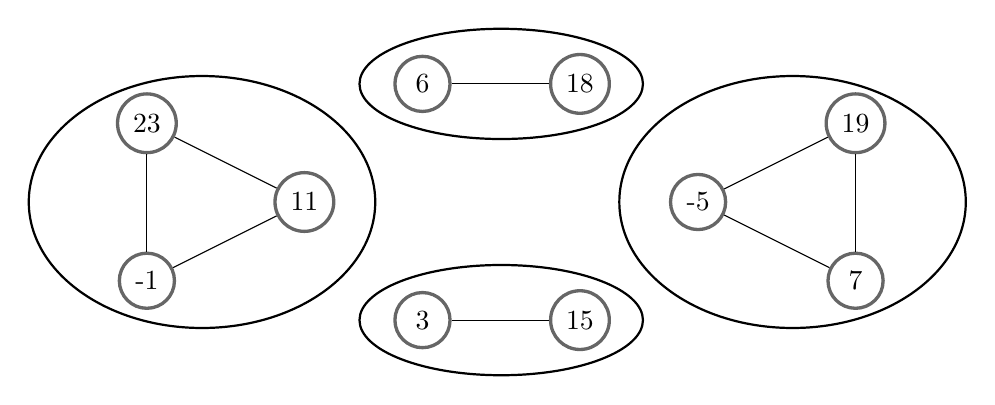
\begin{tikzpicture}[
    node/.style={circle, draw=black!60, very thick, minimum size=7mm},
    ]
    %Nodes
    \node[node] at (-0.5, 0.5) (a) {-1};
    \node[node] at (1.5, 1.5) (b) {11};
    \node[node] at (-0.5, 2.5) (c) {23};
    \node[node] at (6.5, 1.5) (d) {-5};
    \node[node] at (8.5, 0.5) (e) {7};
    \node[node] at (8.5, 2.5) (f) {19};
    \node[node] at (3, 0) (g) {3};
    \node[node] at (5, 0) (h) {15};
    \node[node] at (3, 3) (i) {6};
    \node[node] at (5, 3) (j) {18};
    
    %Lines
    \draw[-] (a) -- (b);
    \draw[-] (a) -- (c);
    \draw[-] (b) -- (c);
    \draw[-] (d) -- (e);
    \draw[-] (d) -- (f);
    \draw[-] (e) -- (f);
    \draw[-] (g) -- (h);
    \draw[-] (i) -- (j);
    
    %elipses
    \draw[thick] (4,0) ellipse (1.8 and 0.7);
    \draw[thick] (4,3) ellipse (1.8 and 0.7);
    \draw[thick] (0.2,1.5) ellipse (2.2 and 1.6);
    \draw[thick] (7.7,1.5) ellipse (2.2 and 1.6);
    \end{tikzpicture}
    \caption{Przykład elementów utożsamionych z sobą w grupie $\mathbb{Z} / 12\mathbb{Z}$, linie oznaczają elementy będące z sobą w relacji równoważności, a elipsy klasy abstrakcji wyznaczone przez tą relację równoważności}
    \label{fig:fourier_vis}
\end{figure}


\subsection{Spojrzenie teorii typów}
Jako że praca skupia się na implementacji typów ilorazowych w Coqu, stąd też bardziej skupimy się na spojrzeniu teorii typów na ilorazy, w przeciwieństwie do spojrzenia teorio mnogościowego. W teorii typów $T/\sim$ będziemy nazywać typem ilorazowym generowanym przez relację równoważności $(\sim)$ na typie pierwotnym $T$. Będziemy oznaczać $a = b$ w typie $T/\sim$ wtedy i tylko wtedy gdy $a \sim b$. Widzimy zatem iż każdy element typ $T$ jest również elementem typu $T/\sim$. Natomiast nie wszystkie funkcje z typu $T$ są dobrze zdefiniowanymi funkcjami z typu $T/\sim$. Funkcja $f: T \rightarrow X$ jest dobrze zdefiniowaną funkcją $f: (T/\sim) \rightarrow X$ jeśli spełnia warunek, że $a \sim b$ implikuje $f(a) = f(b)$. Ten warunek jest konieczny, aby nie dało się rozróżnić utożsamionych wcześniej elementów poprzez zmapowanie ich do innego typu. Myśląc o wszystkich elementach będących z sobą w relacji $(\sim)$ jako o jednym elemencie brak tej zasady spowodowałby złamanie reguły monotoniczności aplikacji mówiącej, że $x = y \Rightarrow f (x) = f (y)$.
\section{Relacje równoważności generowane przez funkcję normalizującą}
Każda funkcja $h: T \rightarrow B$ generuje nam pewną relację równoważności ($\sim_h$) zdefiniowaną poniżej:
\begin{equation}
    \forall x, y \in T, x \sim_h y \iff h(x) = h(y)
\end{equation}
Jak już wspominaliśmy równość jest relacją równoważności, stąd łatwo pokazać iż ($\sim_h$) jest relacją równoważności. Dowolna funkcja $g: B \rightarrow X$ będzie teraz generować dobrze zdefiniowaną funkcję $f: T /\sim_h \rightarrow X$ w taki sposób, że $f = g \circ h$.
\subsection{Funkcja normalizująca}
W tej pracy skupimy się na szczególnym przypadku funkcji $h: T \rightarrow B$ w którym $B = T$. Dodatkowo będziemy wymagać aby funkcja $h$ była idempotentna. Tak zdefiniowaną funkcję h będziemy nazywać funkcją normalizującą.
\begin{code}
\begin{minted}{coq}
Class normalizing_function {A: Type} (f: A -> A) := 
  idempotent : forall x: A, f (f x) = f x.
\end{minted}
\caption{Klasa funkcji normalizujących}
\label{normalizing_function}
\end{code}
Zbudujmy jeszcze odrobinę intuicji wokół tak zdefiniowanych funkcji normalizujących. Jak wiemy relacja równoważności łączny utożsamiane z sobą elementy w grupy, a mówiąc ściślej klasy abstrakcji. Celem funkcji normalizujących jest wyznaczenie reprezentanta każdej z klas abstrakcji. Obrazem tej funkcji będzie właśnie zbór naszych reprezentantów lub inaczej elementów w postaci normalnej. Warunek idempotencji jest konieczny do tego aby obrazem elementu w postaci normalnej był on sam, gdyż nie wymaga on już normalizacji.

\begin{figure}[!htp]
    \centering
    \begin{tikzpicture}[
    node/.style={circle, draw=black!60, very thick, minimum size=0.4}
    ]
    
    %Nodes
    \node[node, double] at (2, 2) (a) {$\frac{1}{2}$};
    \node[node] at (0.5, 3.5) (a0) {$\frac{2}{4}$};
    \node[node] at (3.5, 3.5) (a1) {$\frac{3}{6}$};
    \node[node] at (0.5, 0.5) (a2) {$\frac{10}{20}$};
    \node[node] at (3.5, 0.5) (a3) {$\frac{20}{40}$};

    \node[node, double] at (9, 2) (b) {$\frac{1}{3}$};
    \node[node] at (11.1, 2) (b1) {$\frac{2}{6}$};
    \node[node] at (6.9, 2) (b2) {$\frac{3}{9}$};
    \node[node] at (7.95, 0.2) (b3) {$\frac{4}{12}$};
    \node[node] at (7.95, 3.8) (b4) {$\frac{5}{15}$};
    \node[node] at (10.05, 0.2) (b5) {$\frac{10}{30}$};
    \node[node] at (10.05, 3.8) (b6) {$\frac{6}{18}$};
    
    %Lines
    \path[->, thick] (a) edge [loop above] node {};
    \draw[->, thick] (a0) -- (a);
    \draw[->, thick] (a1) -- (a);
    \draw[->, thick] (a2) -- (a);
    \draw[->, thick] (a3) -- (a);
    
    \path[->, thick] (b) edge [loop above] node {};
    \draw[->, thick] (b1) -- (b);
    \draw[->, thick] (b2) -- (b);
    \draw[->, thick] (b3) -- (b);
    \draw[->, thick] (b4) -- (b);
    \draw[->, thick] (b5) -- (b);
    \draw[->, thick] (b6) -- (b);
    \end{tikzpicture}
    \caption{Przykład działania funkcji normalizującej dla reprezentacji liczby wymiernych w postaci $\mathbb{Z} \times \mathbb{N}$}
    \label{fig:normalizing_function}
\end{figure}

\subsection{Przykłady funkcji normalizujących}
Wykorzystajmy tutaj już wcześniej przytoczony przykład liczb wymiernych. Jednym z sposobów na zdefiniowanie postaci normalnej liczby wymiernej rozumianej jako $\mathbb{Z} \times \mathbb{N}$ jest wymuszenie, aby licznik był względnie pierwszy z mianownikiem. Wprawne oko zapewne zauważy, iż $0$ nie ma kanonicznej postawi w takiej definicji, ale możemy arbitralnie ustalić, że jego postacią normalną będzie $\frac{0}{1}$. W takim przypadku funkcja normalizująca powinna dzielić licznik i mianownik przez ich największy wspólny dzielnik.
W przypadku par nieuporządkowanych, ale na których istnieje jakiś porządek liniowy postacią normalną może być para uporządkowana w której mniejszy element występuje na początku, a funkcją normalizującą będzie funkcja sortująca dwa elementy. Ostatnim, a zarazem najprostszym przykładem niech będzie postać normalna elementów w arytmetyce modularnej o podstawie $m$. Tutaj sama operacja będzie naszą funkcją normalizującą, a więc zostawimy jedynie elementy od zera do $m-1$.   
\section{Typy ilorazowe nie posiadające funkcji normalizujących}
Wykorzystanie funkcji normalizujących w definicji typów ilorazowych jest bardzo wygodne z względu na fakt, że może posłużyć nam do ograniczenia liczby reprezentantów danej klasy abstrakcji do tylko jednego, tego który jest w postaci normalnej. Problem jest jednak to, iż nie każdy typ ilorazowy posiada taką funkcję. W teorii mnogości z aksjomatem wyboru, możemy zawsze wykorzystać ów aksjomat mówiący o tym że z każdej rodziny niepustych zbiorów możemy wybrać zbiór selektorów, w naszym przypadku zbiór elementów w postaci normalnej. Niestety nie możemy skorzystać z niego w Coqowym rachunku indykatywnych konstrukcji. Zobaczmy zatem jakie typy ilorazowe nie są definiowalne w ten sposób
\subsection{Para nieuporządkowana}
Jest to najprostszy typ którego nie można zdefiniować w ten sposób. W żaden sposób nie można określić czy para $\{	\square, \medcircle \}$ jest w postaci normalnej, a może $\{ \medcircle , \square \}$. Oczywiście mając parę wartości na której istnieje pewien porządek zupełny możemy w zbudować parę wykorzystując go. Niestety w ogólności jest to niemożliwe. Niestety wraz z tym idzie iż zbiory, jak i multi-zbiory również nie mają w ogólności swoich postaci kanonicznych, a więc nie można ich zdefiniować dla typów nieposiadających w tym przypadku porządku liniowego.
\subsection{Liczby rzeczywiste definiowane za pomocą ciągów Cauchy'eago}
Kolejnym typem który w spodziewany sposób nie da się znormalizować są liczby rzeczywiste. W Coqu najlepiej je zdefiniować za pomocą ciągów Cauchy'eago liczb wymiernych.
\begin{equation}
    \textbf{isCauchy}(f) := \forall m, n \in \mathbb{N}^+, n < m \rightarrow |f_n - f_m| < \frac{1}{n}
\end{equation}
Granice ciągu będą wyznaczać, którą liczbę rzeczywistą reprezentuje dany ciąg. Chcielibyśmy zatem, aby ciągi o tej samej granicy były z sobą w relacji równoważności. Wyznaczenie granicy ciągu mając jedynie czarną skrzynkę, która może jedynie wyliczać kolejne jej elementy jest niemożliwe. Załóżmy, że jednak jest możliwe, niech $s_k$ będzie ciągiem 1 do k-tego miejsca a później stałym ciągiem 0, natomiast $s_\infty$ ciągiem samych 1. Problem sprawdzenia równości tych ciągów jest przeliczanie rekurencyjny (ciąg $s_k$ może reprezentować zatrzymanie działania programu w $k$-tej sekundzie). Oba ciągi mają różne granice, a co za tym idzie powinny mieć różne postacie normalne, a więc istnieje jakiś element na którym się różnią. Gdyby istniała zatem taka obliczalna i całkowita funkcja normalizująca moglibyśmy za jej pomocą rozwiązać problem stopu w rekurencyjny sposób, sprawdzając jedną wartość ciągu w postaci normalnej. Zatem nie może istnieć taka funkcja.
\subsection{Monada częściowych obliczeń}
Kolejnym typem ilorazowym, dla którego nie może istnieć funkcja normalizująca jest typ częściowych obliczeń. Jak widzimy w definicji \ref{deleyed} jest to typ coinduktywny produkujący albo wynik działania funkcji, albo dalsze obliczenia, które mogą, ale nie muszą się kiedyś skończyć.
\begin{code}
\begin{minted}{coq}
CoInductive delayed (A : Type) := Delayed {
  state : A + delayed A
}.
\end{minted}
\caption{Definicja monady częściowych obliczeń w Coqu.}
\label{deleyed}
\end{code}
W relacji równoważności chcielibyśmy aby były wszystkie obliczenia które ostatecznie zwrócą ten sam wynik, naturalnie będzie istnieć osobna klasa abstrakcji dla obliczeń, które nigdy się nie skończą. Podobnie jednak jak w przypadku powyżej pomimo iż możemy dla każdej klasy abstrakcji wyznaczyć jej reprezentanta w łatwy sposób (obliczenie które natychmiast zwraca wynik), to nie jest to funkcja całkowita rekurencyjna. Możemy zauważyć że za pomocą monady częściowych obliczeń możemy reprezentować dowolne obliczenia wykonywane na maszynie Turinga. Gdyby zatem potrafiliśmy w skończonym czasie wyznaczyć reprezentanta dla każdych obliczeń moglibyśmy w skończonym czasie stwierdzić czy maszyna Turinga się kiedyś zatrzyma, czy też nie. Oznaczało by to rozwiązanie problemu stopu, który jak wiem jest problemem nie rekurencyjnym. 


	
    \chapter{Quotient types and subtypes}
	\section{Subtyping}
\begin{defi}{Subtypes}{def:subtypes}
A \emph{subtype} $A \sqsubseteq B$ is a type that contains a specific subset of elements of the underlying type $B$.
\end{defi}
\begin{example}{}{ex:subtype}
A great example of a subtype is the type of even numbers, a subtype of natural numbers.
\end{example}
Subtyping is a pretty intuitive concept. However, subtyping in Coq can be tricky for users accustomed to object-oriented languages like Java \cite{Java}. In such languages, subtyping is usually associated with the concept of inheritance and is used to define polymorphic construction. In other words, we can use an element for a subtype when an element of the underlying type is required. Similarly, in math, we expect an even number to be a natural number. Unfortunately, such intuitions do not apply in Coq.
\begin{defi}{Subtypes in Coq}{def:siq}
\begin{minted}{coq}
Inductive sig (A : Type) (P : A -> Prop) : Type :=
    exist : forall x : A, P x -> sig P.
\end{minted}
\end{defi}
\begin{defi}{Subtypes in Coq using record}{def:siq'}
\begin{minted}{coq}
Record sig' (A : Type) (P : A -> Prop) : Type := exist' {
    proj1' : A;
    proj2' : P proj1';
}
\end{minted}
\end{defi}
Subtypes in Coq can be defined in two equivalent ways (see definitions \ref{def:siq} and \ref{def:siq'}). The first definition is used in Coq's standard library. The second one nicely shows that a subtype is actually a dependent pair built of two elements, a value, and  the proof that the value satisfies a specific predicate.
\begin{defi}{Depandent pair}{def:dep_pair}
\emph{Dependent pair} is a generalization of pair where the type of the second element depends on the value of the first one.
\end{defi}
\begin{example}{}{ex:dep_pair}
An example of a dependent pair type is the type of pairs of two coprime numbers. The value of the first element determines the type of the second element. For example, if the first element is five, the second element must be a number coprime to five.
\end{example}
Since subtypes are defined as dependent pairs in Coq, we cannot use an element of the subtype as an element of the underlying type. However, in contrast to the majority of programming languages in Coq, we can use subtypes to define concepts like the type of sorted lists and, for example, use this type as a type of argument of the binary search function. The benefits of such function types are obvious for developing reliable software.
\begin{coq}{The notation for subtyping}{coq:subtype_notation}
In Coq, there is a special notation for subtypes: \mcoq{{a : A | P a}} that should resemble mathematical notation for $\{a \in A: P(a)\}$.
\end{coq}
\begin{example}{The subtype of natural numbers less than 10}{ex:lessThanTen}
\begin{minted}{coq}
Definition lessThanTen := {a : nat | a < 10}.
\end{minted}
\end{example}
\subsection{Connetion to quotient types}
Subtyping is the dual construction of quotient types. As mentioned in the introduction, there is no a built-in method for implementing quotient types in Coq. Therefore, we will use subtypes to define types containing only normalized elements of the underlying type. The normalized elements are defined as the image of some normalization function. This construction defines a type where equality is equivalent to a quotient-defining equality relation because every equivalence class is reduced to single element.
\begin{defi}{Subtype of normalized elements}{def:subtype_quot}
\begin{minted}{coq}
Record quotient {A: Type} (f: A -> A) `{normalization f} := {
  val: A;
  valIsNormal: val = f val
}.
\end{minted}
\end{defi}
\section{Duality}
In the previous section, we mentioned that subtyping is a dual concept to quotient types. This optional section explains what it means and why it is the case. Knowledge about category theory would improve the reading experience. However, this part is more of an interesting fact than an integral part of this work, so feel free to skip it.
\begin{defi}[]{Duality}{def:dual}
In category theory, the statement dual to $\sigma$ is denoted as $\sigma^{\textrm{op}}$ and defined by \cite{CategoryTheory}:
\setlist{nolistsep}
\begin{itemize}
    \itemsep 0em 
    \item interchanging the source and target of each morphism in $\sigma$
    \item interchanging the order of composing two morphisms in $\sigma$ 
\end{itemize}
\end{defi}

\begin{vis}[]{Product and coproduct}{vis:dual}
The formal definition of duality might take much effort to understand. A visual example of two dual constructions should give enough insight to comprehend this concept. On the left side, we see a product, and on the right side, a dual construction to product, known as a coproduct.
\begin{center}
    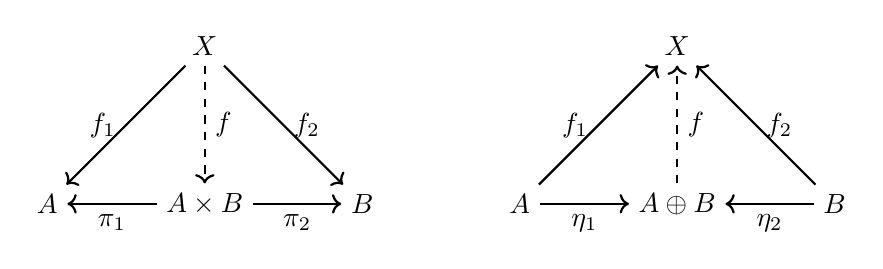
\begin{tikzpicture}[node/.style={circle, draw=black!60, very thick, minimum size=0.4}]
    %Nodes
    \node[] at (0, 0) (pA) {$A$};
    \node[] at (4, 0) (pB) {$B$};
    \node[] at (2, 2) (pX) {$X$};
    \node[] at (2, 0) (pS) {$A \times B$};
    
    \node[] at (6, 0) (cA) {$A$};
    \node[] at (10, 0) (cB) {$B$};
    \node[] at (8, 2) (cX) {$X$};
    \node[] at (8, 0) (cS) {$A \oplus B$};
    
    %Lines
    \draw[->, thick] (pS) -- (pA) node [below, midway] {$\pi_1$};
    \draw[->, thick] (pS) -- (pB) node [below, midway] {$\pi_2$};
    \draw[->, thick] (pX) -- (pA) node [left, midway] {$f_1$};
    \draw[->, thick] (pX) -- (pB) node [right, midway] {$f_2$};
    \draw[->, thick, dashed] (pX) -- (pS) node [right, midway] {$f$};
    
    \draw[->, thick] (cA) -- (cS) node [below, midway] {$\eta_1$};
    \draw[->, thick] (cB) -- (cS) node [below, midway] {$\eta_2$};
    \draw[->, thick] (cA) -- (cX) node [left, midway] {$f_1$};
    \draw[->, thick] (cB) -- (cX) node [right, midway] {$f_2$};
    \draw[->, thick, dashed] (cS) -- (cX) node [right, midway] {$f$};
    
    \end{tikzpicture}
\end{center}
Both diagrams commute, meaning that all directed paths in the diagram with the same start and endpoints lead to the same result \cite{CategoryTheory}.
\end{vis}
In other words, we can construct a dual concept by reversing each arrow (morphism) in the diagram. However, definitions of subtyping and quotient types
do not seems to have any arrows. In order to find them, we need to look into pushouts and pullbacks constructions known from category theory \cite{CategoryTheory}.
\subsection{Pushout}
\begin{defi}{Pushout}{def:pusout}
The \emph{pushout} \cite{CategoryTheory} $P$ is defined by two morphisms $f: X \rightarrow A$ and $g: X \rightarrow B$, with common domain $X$.
\begin{center}
    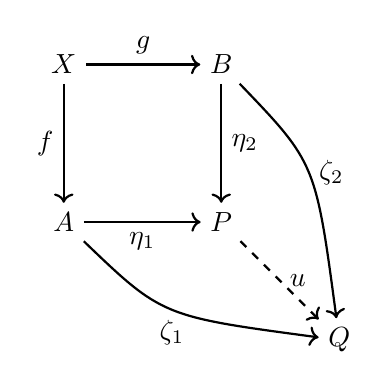
\begin{tikzpicture}[node/.style={circle, draw=black!60, very thick, minimum size=0.4}]
    %Nodes
    \node[] at (0, 0) (a) {$A$};
    \node[] at (2, 0) (p) {$P$};
    \node[] at (0, 2) (x) {$X$};
    \node[] at (2, 2) (b) {$B$};
    
    \node[] at (3.5, -1.5) (q) {$Q$};
    
    %Lines
    \draw[->, thick] (x) -- (a) node [left, midway] {$f$};
    \draw[->, thick] (x) -- (b) node [above, midway] {$g$};
    \draw[->, thick] (a) -- (p) node [below, midway] {$\eta_1$};
    \draw[->, thick] (b) -- (p) node [right, midway] {$\eta_2$};
    \draw[->, thick] (a) .. controls +(1.25, -1.2) .. (q) node [below, midway] {$\zeta_1$};
    \draw[->, thick] (b) .. controls +(1.2, -1.25) .. (q) node [right, midway] {$\zeta_2$};
    \draw[->, thick, dashed] (p) -- (q) node [right, midway] {$u$};
    
    \end{tikzpicture}
\end{center}
The pushout $P$ is an object along with two morphisms $\eta_1: A \rightarrow P$ and $\eta_2: B \rightarrow P$ that complete commutative square with two given morphisms $f: X \rightarrow A$ and $g: X \rightarrow B$. However, not every object that makes the square commutative is a pushout. The pushout must be the "most general" way to complete the commutative square. By the "most general" way, we mean that for every other object Q, which also completes commutative square with two morphisms $\zeta_1: A \rightarrow Q$ and $\zeta_2: B \rightarrow Q$, a unique morphism $u: P \rightarrow Q$ must exist that makes the whole diagram commutative. Not for all morphisms $f: X \rightarrow A$ and $g: X \rightarrow B$, pushout exists, but if it exists, it is unique up to the unique isomorphism.
\end{defi}
The pushout is a useful concept in category theory, but its connection to quotient types is not obvious. To see this connection let us take a trip to the world of \emph{Set} category. In this category, sets are objects, and functions between sets are morphisms. We will show that, indeed, in this category, quotient types are pushouts. On the diagram of the pushout definition, we can see that $A$, $B$, and $P$ define something in the shape of a coproduct. Let us use coproduct $A \oplus B$ as a base for the pushout definition and let functions $\eta_1: A \rightarrow A \oplus B$ and $\eta_2: B \rightarrow A \oplus B$ be natural injections. For $A \oplus B$ to be pushout, we also need to ensure that $X$, $A$, $B$ and $A \oplus B$ are commutative square, that means for every $x \in X$ following should be true $\eta_1(f(x)) = \eta_2(g(x))$. In order to achieve that, we need to modify $A \oplus B$, by gluing together injections of $f(x)$ and $g(x)$ in $A \oplus B$. As we know, gluing together elements means defining the quotient type $P = ((A \oplus B) / \sim)$, where for every $x \in X$ $f(x) \sim g(x)$. For $P = ((A \oplus B) / \sim)$ to be a pushout, we need to define $(\sim)$ as the largest in terms of equivalence classes relation that completes the commutative square. 
\begin{theo}{}{th:pushout}
If there exists a larger equivalence relation $(\simeq)$ that $X$, $A$, $B$, and $Q = ((A \oplus B
)/\simeq)$ also commutes, then there cannot exist a unique morphism $u: P \rightarrow Q$ that makes whole diagram commutative. 
\end{theo}

\begin{proof}{}{proof:pushout}
Since $|Q| > |P|$, morphism $u$ cannot be a surjection it follows that there exist $y \in Q$ such that for all  $x \in P$ $u(x)$ is not equal to $y$. 
Without loss of generality exists $a \in A$ such that $\zeta_1(a) = y$. From commutivity we know that $\zeta_1(a) = u(\eta_1(a))$, but $\eta_1(a) \in P$. \contradiction
\end{proof}

\begin{example}{Circle defined by a pushout}{ex:circ}
In category \emph{Set}, we can use a pushout to construct a circle out of two bounded lines $[0, 1]$. Let us define two morphisms $f: \{0, 1\} \rightarrow  [0, 1]$ and $g: \{0, 1\} \rightarrow  [0, 1]$ as identity functions. Let $C$ be pushout defined by such morphisms.

\begin{center}
    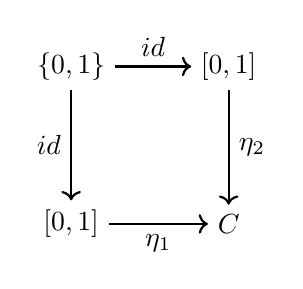
\begin{tikzpicture}[node/.style={circle, draw=black!60, very thick, minimum size=0.4}]
    %Nodes
    \node[] at (0, 0) (a) {$[0, 1]$};
    \node[] at (2, 0) (p) {$C$};
    \node[] at (0, 2) (x) {$\{0, 1\}$};
    \node[] at (2, 2) (b) {$[0, 1]$};
    
    %Lines
    \draw[->, thick] (x) -- (a) node [left, midway] {$id$};
    \draw[->, thick] (x) -- (b) node [above, midway] {$id$};
    \draw[->, thick] (a) -- (p) node [below, midway] {$\eta_1$};
    \draw[->, thick] (b) -- (p) node [right, midway] {$\eta_2$};;
    
    \end{tikzpicture}
\end{center}
Let us check if $C$ is a circle. Since the diagram above commutes then, we know that $\eta_1(0) = \eta_2(0)$ and $\eta_1(1) = \eta_2(1)$ so, we glued together two points. Moreover, we know that $C$ is defined by the equivalence relation largest in terms of equivalence classes. Therefore every other point of both bounded lines has to have a natural injection into $C$. Based on this, we can conclude that $C$ represents a circle. This construction can be generalized for $n$-dimensional hyper-spheres. Gluing together two $n$-dimensional hemispheres alongside $(n-1)$-dimensional sphere, gives a $n$-dimmensional sphere.
\end{example}

\subsection{Pullback}
Knowing that a pullback is a dual construction to pushout and knowing what dual construction is, everyone should be able to draw a pushout defining diagram.
\begin{defi}{Pullback}{def:pullback}
The pullback \cite{CategoryTheory} $P$ is defined by two morphisms $f: A \rightarrow X$ and $g: B \rightarrow X$, with common codomain $X$.
\begin{center}
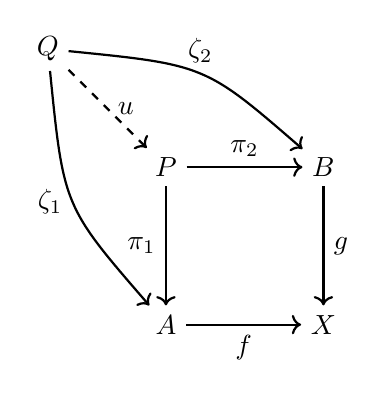
\begin{tikzpicture}[node/.style={circle, draw=black!60, very thick, minimum size=0.4}]
    %Nodes
    \node[] at (0, 0) (a) {$A$};
    \node[] at (0, 2) (p) {$P$};
    \node[] at (2, 0) (x) {$X$};
    \node[] at (2, 2) (b) {$B$};
    
    \node[] at (-1.5, 3.5) (q) {$Q$};
    
    %Lines
    \draw[->, thick] (a) -- (x) node [below, midway] {$f$};
    \draw[->, thick] (b) -- (x) node [right, midway] {$g$};
    \draw[->, thick] (p) -- (a) node [left, midway] {$\pi_1$};
    \draw[->, thick] (p) -- (b) node [above, midway] {$\pi_2$};
    \draw[->, thick] (q) .. controls +(0.2, -2) .. (a) node [left, midway] {$\zeta_1$};
    \draw[->, thick] (q) .. controls +(2, -0.2) .. (b) node [above, midway] {$\zeta_2$};
    \draw[->, thick, dashed] (q) -- (p) node [right, midway] {$u$};
    
    \end{tikzpicture}
\end{center}
The pullback $P$ is an object along with two morphisms $\pi_1: P \rightarrow A$ and $\pi_2: P \rightarrow B$ that complete commutative square with two given morphisms $f: A \rightarrow X$ and $g: B \rightarrow X$. However, not every object that makes the square commutative is a pullback. The pullback must be the "most general" way to complete the commutative square. By the "most general" way, we mean that for every other object Q, which also completes commutative square with two morphisms $\zeta_1: Q \rightarrow A$ and $\zeta_2: Q \rightarrow B$, a unique morphism $u: Q \rightarrow P$ must exist that makes the whole diagram commutative. Not for all morphisms $f: A \rightarrow X$ and $g: B \rightarrow X$, pullback exists, but if it exists, it is unique up to the unique isomorphism.
\end{defi}
In order to understand the connection between a pullback and subtyping, we again take a trip to the \emph{Set} category. As expected in dual construction, in the pullback $A$, $B$, and $P$ are in the shape of a product. Therefore, let us use product $A \times B$ as the base for the pushout definition and let functions $\pi_1: A \times B \rightarrow A$ and $\pi_2: A \times B \rightarrow B$ be natural projections. In order to complete the commutative square for every $p \in A \times B$, the following needs to be true $f (\pi_1 (p)) = g (\pi_2(p))$. Therefore, we need to use the following subset $P = \{(a, b) \in A \times B : f(a) = g(b)\}$. 
\begin{theo}{}{th:pulback}
For every other subset $Q \subseteq A \times B$ and two morphisms $\zeta_1: Q \rightarrow A$ and $\zeta_1: Q \rightarrow B$ that completes the commutative square, there exists a unique morphism $u: Q \rightarrow P$ makes the whole diagram commutative.
\end{theo}
\begin{proof}{}{proof:pullback}
Let define $u(q) = (\zeta_1(q), \zeta_2(q))$. Since $\pi$ functions are simple projections the following is true $\zeta_1 = \pi_1 \circ u$ and $\zeta_2 = \pi_2 \circ u$. \qed
\end{proof}
\begin{example}{Pairs of natural numbers of this same parity}{ex:parity_pair}
In category \emph{Set}, we can use the pullback to define the set of pairs of integers with this same parity. Let us define morphism $f(n) = n \; \textrm{mod} \; 2$ that checks the parity of an integer.
\begin{center}
    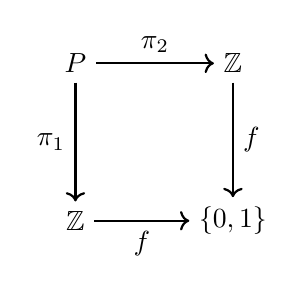
\begin{tikzpicture}[node/.style={circle, draw=black!60, very thick, minimum size=0.4}]
    %Nodes
    \node[] at (0, 0) (a) {$\mathbb{Z}$};
    \node[] at (0, 2) (p) {$P$};
    \node[] at (2, 0) (x) {$\{0, 1\}$};
    \node[] at (2, 2) (b) {$\mathbb{Z}$};
    
    %Lines
    \draw[->, thick] (a) -- (x) node [below, midway] {$f$};
    \draw[->, thick] (b) -- (x) node [right, midway] {$f$};
    \draw[->, thick] (p) -- (a) node [left, midway] {$\pi_1$};
    \draw[->, thick] (p) -- (b) node [above, midway] {$\pi_2$};;
    
    \end{tikzpicture}
\end{center}
As we know, the "most general" $P$ that completes this commutative square is $\{(n, m) \in \mathbb{Z} \times \mathbb{Z} : n \equiv_2 m\}$.
\end{example}
\subsection{Conclusion}
As shown in the examples above, the pushout can define quotient types in category theory, and the pullback can be used to define subtypes.  Those two constructions are mutually dual. Therefore we can call subtyping a dual concept to quotients types.
\section{Uniquness of representation}
In Coq, subtyping is realized using dependent pairs of value and proof that the value satisfies the subtype defining predicate. Unfortunately, this means that only some properties of subtypes known from mathematics hold in Coq. As mentioned at the beginning of this chapter, we cannot use a member of a subtype as a member of the underlying type. This particular problem is easy to fix using projections. The other consequence of using dependent pair related to using subtyping as quotient types is that we cannot prove that only one member of subtype exists for every value that satisfies the subtype defining predicate. As we know irrelevance of proofs is independent of axioms of the \mcoq{Prop} universe \cite{CoqBook2}. It is a major problem since we want to use subtyping to reduce each equivalence class to a single element. The possibility of the existence of multiple elements that only differ by proof of subtype defining predicate makes this construction useless for quotient types applications. Hence, we need to define the subset of quotient types for which its subtype representations are unique or redefine this construction for these purposes.
\begin{defi}{Class of subtypes with unique represenations}{def:unique_representation}
\begin{minted}{coq}
Class unique_representation {A: Type} (P: A -> Prop) := 
  { uniq : forall (x y : {a : A | P a}), 
    proj1_sig x = proj1_sig y -> x = y }.
\end{minted}
\end{defi}
\begin{coq}{}{coq:proj1_sig}
In coq function \mcoq{proj1_sig} is a projection of the subtype value. It can be thought of as a lifting to the underlying type.
\end{coq}
\subsection{Axiomatic approach}
As mentioned in the introduction, we avoid using axioms in this paper. However, it is worth considering their effect on this problem and if it is safe to use them.
\subsubsection{Proof irrelevance axiom}
Proof irrelevance is a known concept in computer science \cite{ProofIrrelevance}. It states that every two proofs of this same statement are equal.
\begin{defi}{Axiom of proof irrelevance}{def:proof_irrelevance}
\begin{minted}{coq}
Definition Irrelevance := forall (P: Prop) (x y: P), x = y.
\end{minted}
\end{defi}
Using this axiom, we can easily prove that every subtype has unique representation (as defined in \ref{def:unique_representation}).
\begin{theo}{}{th:irr_uniq}
    \begin{minted}{coq}
Theorem irrelevance_impl_unique_representation : Irrelevance -> 
  forall (A: Type) (P: A -> Prop), unique_representation P.
    \end{minted}
\end{theo}
\begin{proof}{}{proof:irr_uniq}
    \begin{minted}{coq}
intros Irr A P. constructor. intros [x xp] [y yp] H.
cbn in H. subst.
Require Import Coq.Logic.EqdepFacts.
apply eq_dep_eq_sig.
specialize (Irr (P y) xp yp); subst.
constructor. Qed.
\end{minted}
\end{proof}
Those two statements are equivalent. Thus, the axiom of proof irrelevance is required for every subtype to have a unique representations.
\begin{theo}{}{th:irr_uniq2}
    \begin{minted}{coq}
Theorem unique_representation_impl_irrelevance : 
  (forall (A: Type) (P: A -> Prop), unique_representation P) -> 
  Irrelevance.
    \end{minted}
\end{theo}
\begin{proof}{}{proof:irr_uniq2}
    \begin{minted}{coq}
intros Uniq P x y.
specialize (Uniq unit (fun _ => P)). destruct Uniq as [Uniq].
specialize (Uniq (exist _ tt x) (exist _ tt y) eq_refl).
Require Import Coq.Logic.Eqdep_dec.
refine (eq_dep_eq_dec (A := unit) _ _).
- intros. left. destruct x0, y0. reflexivity.
- apply eq_sig_eq_dep. apply Uniq. Qed.
\end{minted}
\end{proof}
\begin{coq}{Dependent equality}{coq:eq_dep}
In coq, \emph{dependent equality} is defined as:
\begin{minted}{coq}
Inductive eq_dep (U : Type) (P : U -> Type) (p : U) (x : P p) 
  : forall q : U, P q -> Prop :=
    eq_dep_intro : eq_dep U P p x p x.
\end{minted}
Proofs above use additional theorems \mcoq{eq_dep_eq_sig} state that if two values as dependently equal, then subtypes made of them are equal. The second one, \mcoq{eq_sig_eq_dep}, states that for types with decidable equality, dependent equality implies equality.
\end{coq}

\subsubsection{Axiom K}
Axiom K (also known as Uniqueness of Identity Proof) is a weaker version of the proof irrelevance axiom. It states that two proofs of this same equality are equal. Thomas Streicher first introduced it in his habilitation thesis \cite{Streicher}.
\begin{defi}{Axiom K}{def:axiom_K}
\begin{minted}{coq}
Definition K := forall (A: Type) (x y: A) (p q: x = y), p = q.
\end{minted}
\end{defi}
\begin{coq}{Embedding dependent equality in equality}{coq:eq_emb}
Interesting consequence of using axiom K is that it embeds dependent equality in equality.
\begin{minted}{coq}
Fact eq_dep_embedded_in_eq : forall (A : Type) (P : A -> Prop)
  (a : A) (p q : P a), eq_dep A P a p a q -> p = q.
\end{minted}
Proof of this fact is outside the scope of this section, but it can be found in \coqsource{Extras/Stricher.v}.
\end{coq}
Since axiom K is weaker than the proof irrelevance axiom, we cannot prove that every subtype is a class of unique representations. However, we can use it to prove that every quotient (defined in \ref{def:subtype_quot}) has unique representations.
\begin{theo}{}{th:subtype_quot_uniq}
\begin{minted}{coq}
Theorem quotient_unique_representation: K -> forall (A: Type) 
  (f: A -> A) `{normalization A f} (x y : quotient f),
  val x = val y -> x = y.
\end{minted}
\end{theo}
\begin{proof}{}{proof:subtype_quot_uniq}
\begin{minted}{coq}
intros K A f N [x xp] [y yp] H. 
cbn in *. subst. 
specialize (K _ _ _ xp yp). subst. 
reflexivity. Qed.
\end{minted}
\end{proof}
\subsection{Definitional irrelevance approach}
As mentioned in this section, we can add the axiom of proof irrelevance to solve the problem of unique representations for every subtypes. In Coq, there is another approach to proof irrelevance - \mcoq{SProp}.
\begin{coq}[]{\mcoq{SProp} universe}{coq:SProp}
\mcoq{SProp} (Strict Propositions) is a universe of propositions with definitional proof irrelevance as described in \cite{BasesOfSProp}. It is still an experimental feature\cite{coqDoc} of Coq and requires work to be fully functional. The standard library of Coq has several useful constructions for strict propositions:
\begin{description}
    \item \mcoq{Box} -- a record that lifts \mcoq{SProp} proposition to \mcoq{Prop} universe.
    \begin{minted}{coq}
Record Box (A : SProp) : Prop := box { unbox : A }.
    \end{minted}
    \item \mcoq{Squash} -- an inductive type that squashes proposition into \mcoq{SProp} universe making it proof irrelevant.
    \begin{minted}{coq}
Inductive Squash@{u} (A : Type) : SProp :=  
  squash : A -> Squash A.
    \end{minted}
    \item \mcoq{sEmpty} -- an equivalent of \mcoq{False} in \mcoq{Prop}. From \mcoq{sEmpty} anything follows.
    \begin{minted}{coq}
Inductive sEmpty@{} : SProp :=  .
Definition sEmpty_rect : forall (P : sEmpty -> Type) 
  (s : sEmpty), P s.
    \end{minted}
    \item \mcoq{sUnit} -- an equivalent of \mcoq{True} in \mcoq{Prop}.
    \begin{minted}{coq}
Inductive sUnit@{} : SProp :=  stt : sUnit.
    \end{minted}
    \item \mcoq{Ssig} -- subtype defined in \mcoq{SProp} universe.
    \begin{minted}{coq}
Record Ssig (A : Type) (P : A -> SProp) : Type :=
  Sexists { Spr1 : A;  Spr2 : P Spr1 }.
    \end{minted}
\end{description}
\end{coq}
We can easily prove that subtypes defined using \mcoq{Ssig} have unique representations.
\begin{theo}{}{th:ssig}
\begin{minted}{coq}
Theorem Ssig_unique_representation : forall (A : Type) 
  (P : A -> SProp) (a b : Ssig P), Spr1 a = Spr1 b -> a = b.
\end{minted}
\end{theo}
\begin{proof}{}{proof:ssig}
\begin{minted}{coq}
intros A P [a ap] [b bp] H.
cbn in *. subst.
reflexivity. Qed.
\end{minted}
\end{proof}
Using \mcoq{Ssig} is very convenient since having unique representations does not require additional axioms. However, the disadvantage of this approach is that the proof that the value satisfies the subtype defining predicate is in the \mcoq{SProp} universe. Therefore, using this proof in the \mcoq{Prop} universe, where most theorems live, is usually impossible. The only exception is when we can use it to prove \mcoq{sEmpty}.
\subsection{Homotopic approach}
If we want to work in the \mcoq{Prop} universe without additional axioms, we must find underlying types with unique identity poofs. It is a challenging task. Nevertheless, with help comes Homotopy Type Theory (HoTT) \cite{HoTT}. It is a relatively new Type Theory branch focusing on identity proofs. Homotopic interpretation of a type is $\omega$-grupoid. In such groupoid, nodes represent members of a type; paths represent identity proofs; paths between paths represent identity proofs of identity proofs, and so forth. 
\subsubsection{Homotopy $n$-types}
Homotopy $n$-types creates a type hierarchy based on the complexity of identity poofs structure ($\omega$-grupoid structure).
\begin{example}{Selected $n$-types}{ex:n_types}
Developing intuition regarding this concept is important before formally defining the $n$-th type. Therefore, we will discuss the three most important examples of $n$-types for this thesis.
\begin{description}
    \item \mcoq{Contr} -- it is the lowest minus-second universe. The type that lives in \mcoq{Contr} has exactly one element. A good example of $(-2)$-type is a \mcoq{unit}.
    \begin{minted}{coq}
 Class isContr (A: Type) := ContrBuilder {
   center : A;
   contr  : forall x: A, x = center
 }.
    \end{minted}
    \item \mcoq{HProp} -- it is the minus-first universe. Not to be confused with Coq's \mcoq{Prop}. The type that lives in it has every element equal to each other. A good example of $(-1)$-type is \mcoq{Empty_set}. We can easily prove that each element of the empty type is the same element. However, it has no elements, so it cannot live in \mcoq{Contr}.
        \begin{minted}{coq}
 Class isHProp (P : Type) :=
   hProp : forall p q : P, p = q.
    \end{minted}
    \item \mcoq{HSet} -- it is the zero universe. Not to be confused with Coq's \mcoq{Set}. The type that lives in it has unique identity proofs. A good example of $0$-type is \mcoq{boo}l. We will later in this section show that it has unique identity proofs. Moreover, it has two elements, so it does not live in \mcoq{HProp}.
    \begin{minted}{coq}
 Class isHSet (X : Type) :=
   hSet : forall (x y : X) (p q : x = y), p = q.
    \end{minted}
\end{description}
\end{example}
\begin{defi}{$N$-th type}{def:nth_type}
\begin{minted}{coq}
Inductive universe : Type :=
| minus_two  : universe
| S_universe : universe -> universe.

Fixpoint isNType (n : universe) (A : Type) : Type :=
match n with
| minus_two => isContr A
| S_universe n' => forall x y: A, isNType n' (x = y)
end.
\end{minted}
\end{defi}
As we see in the definition, $n$-types are defined by where identity proofs of elements of those types live. The hierarchy starts at the $(-2)$-type, where only the most primitive contactable types live. Types with identity proofs in \mcoq{Contr} live in \mcoq{HProp} since the identity proof type is inhabited for every pair of elements. Therefore, every two elements are equal. Similarly, if identity proofs of type live in \mcoq{HProp}, then the type lives in \mcoq{HSet} since, for every two elements, in the type of identity proofs, every two elements are equal. The other important fact is that every $n$-type is also a $(n+1)$-type.
\begin{theo}{$n$-type inclusion}{th:nth_incl}
\begin{minted}{coq}
Theorem NType_inclusion : forall A: Type, forall n : universe,
  isNType n A -> isNType (S_universe n) A.
\end{minted}
\end{theo}
\begin{proof}{}{proof:nth_incl}
Proof of this theorem can be found in \coqsource{Lib/HoTT.v}.
\end{proof}
\subsubsection{Types with decidable equality}
If the underlying type of quotient (defined in \ref{def:subtype_quot}) lives in the \mcoq{HSet} universe, then we can easily prove that it has a unique representation the same way as in proof \ref{proof:subtype_quot_uniq}. However, proving that a type lives in \mcoq{HSet} is not trivial. Fortunately, Hedberg's theorem \cite{hedberg_1998} gives us a valuable sufficiency condition -- decidable equality.
\begin{defi}{Decidable equality}{def:dec_eq}
\begin{minted}{coq}
Class Decidable (A : Type) :=
  dec : A + (A -> False).
  
Class DecidableEq (A : Type) :=
  dec_eq : forall x y: A, Decidable (x = y).
\end{minted}
\end{defi}
For type be have decidable equality means that there exists an algorithm that, a finite amount of time, decides if two elements of this type are equal.
\begin{theo}{Hedberg's theorem}{th:hedberg}
\begin{minted}{coq}
Theorem hedberg (A : Type) : EqDec A -> isHSet A.
\end{minted}
\end{theo}
\begin{proof}{}{proof:hedberg}
This proof of Hedberg's theorem is based on the paper \cite{HedbergProof}. It is based on the concept of collapsibility.
\begin{minted}{coq}
Class Collapsible (A : Type) := { 
  collapse        : A -> A ;
  wconst_collapse : forall x y: A, collapse x = collapse y;
}.
\end{minted}
It can be easily proven that the type is collapsible if it is decidable.
\begin{minted}{coq}
Theorem dec_is_collaps : forall A : Type, Decidable A -> 
  Collapsible A.
Proof.
  intros A eq. destruct eq.
  - exists (fun x => a). intros x y. reflexivity.
  - exists (fun x => x); intros x y.
    exfalso; apply f; assumption.
Qed.
\end{minted}
This same law applies to the type of identity proofs.
\begin{minted}{coq}
Class PathCollapsible (A : Type) :=
  path_coll : forall (x y : A), Collapsible (x = y).

Theorem eq_dec_is_path_collaps : forall A : Type, 
  DecidableEq A -> PathCollapsible A.
Proof.
  intros A dec x y. apply dec_is_collaps. apply dec.
Qed.
\end{minted}
We need a simple lemma about composition identity proofs.
\begin{minted}{coq}
Lemma loop_eq : forall A: Type, forall x y: A, forall p: x = y, 
  eq_refl = eq_trans (eq_sym p) p.
Proof.
  intros A x y []. cbn. reflexivity.
Qed.
\end{minted}
Using the lemma above, we can prove that type with collapsable paths lives in \mcoq{HSet}.
\begin{minted}{coq}
Theorem path_collaps_is_hset (A : Type) : PathCollapsible A -> 
  isHSet A.
Proof.
  unfold isHSet, PathCollapsible; intros C x y.
  cut (forall e: x=y, e = 
    eq_trans (eq_sym(collapse(eq_refl x))) (collapse e)).
  - intros H p q. 
    rewrite (H q), (H p), (wconst_collapse p q).
    reflexivity.
  - intros []. apply loop_eq.
Qed.
\end{minted}
Composing \mcoq{dec_is_collaps} with \mcoq{path_collaps_is_hset}, we get proof that every type with decidable equality lives in \mcoq{HSet} and has only trivial paths. \qed
\end{proof}
Hedberg's theorem shows that every quotient (defined in \ref{def:subtype_quot}) with an underlying type with decidable equality has unique representations. Since to define such quotient (defined in \ref{def:subtype_quot}), we need to define normalization function (defined in \ref{def:normalization_function}) that should not be an issue.
\subsubsection{Characterization of dependent pair equality}
\begin{coq}{Dependent pair}{coq:dep_pair}
In Coq, the type of \emph{dependant pair} is defined using inductive type.
\begin{minted}{coq}
Inductive sigT (A : Type) (P : A -> Type) : Type :=
  existT : forall x : A, P x -> sigT A P.
\end{minted}
\mcoq{{x : A & P x}} is the notation for dependent pairs.
\end{coq}
Subtypes are based on dependent pairs. Therefore, knowing how the equality of dependent pairs can be characterized is worthwhile. In the case of simple nondependent pairs, the characterization is straightforward.
\begin{theo}{Characterization of pair equality}{th:pair_eq}
\begin{minted}{coq}
Theorem pair_eq : forall (A B: Type) (a x : A) (b y : B),
  (a, b) = (x, y) -> a = x /\ b = y.
\end{minted}
\end{theo}
\begin{proof}{}{proof:pair_eq}
\begin{minted}{coq}
intros. inversion H. split; trivial. Qed.
\end{minted}
\end{proof}
Using this same definition for dependent pairs is impossible. The first issue is the error of ill-defined equality since P x and P y differ in the Coq type system, even if x = y, and elements of two different types cannot be in equality relation. Even if we redefine our problem to the characterization of equality for dependent pairs with this same first element, it is still impossible to characterize it using simple equality. Such equality can be characterized using dependent equality known from Coq's fact \ref{coq:eq_dep}. Moreover, from Coq's fact \ref{coq:eq_emb}, we know that for characterization using simple equality to be correct, the axiom K must be added. To characterize the general case of dependent pairs equality, we need first to define transport of equality path.
\begin{defi}{Transport}{def:transport}
\begin{minted}{coq}
Definition transport {A: Type} {a b: A} {P: A -> Type} 
  (p: a = b) (x : P a) : P b :=
match p with
| eq_refl => x
end.
\end{minted}
\end{defi}
Transport construction moves an element of type \mcoq{P a} to a new type  \mcoq{P b} along the path (proof of equality) \mcoq{p: a = b}. Using this construction, we can characterize equality for dependent pairs.
\begin{vis}[G]{Transport}{vis:transport}
$P$ is a family of types indexed by elements of type $A$. Two elements, $a$ and $b$, are equal in $A$, and $p$ is a proof of this fact (path). Element $x$ of type $P(a)$ can be transported along this proof (path) to type $P(b)$.
\begin{center}
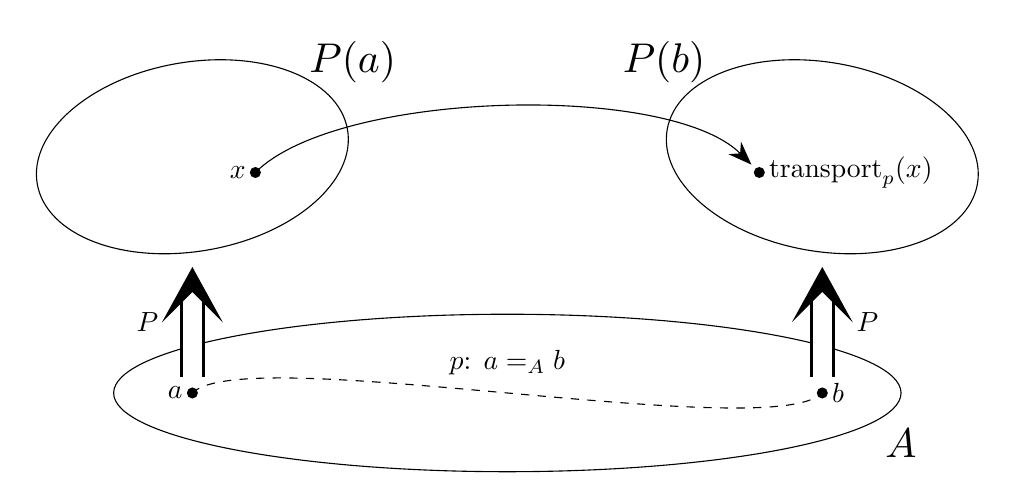
\begin{tikzpicture}
    \draw (0,0) circle [x radius=5cm, y radius=1cm];
    \fill (5, -1) circle (0pt) node[above, scale=1.5] {$A$};
    \draw (-4,3) circle [x radius=2cm, y radius=1.2cm, rotate=10];
    \fill (-2.7,4.2) circle (0pt) node[above, right,scale=1.5] {$P(a)$};
    \draw (4,3) circle [x radius=2cm, y radius=1.2cm, rotate=-10];
    \fill (2.7,4.2) circle (0pt) node[above, left,scale=1.5] {$P(b)$};
    \draw [line width=1pt, double distance=7pt,
             arrows = {-Stealth[length=20pt, inset=11pt, width=22pt]}] (4,0.2) -- (4,1.6) node[midway, right=3mm]{$P$};
    \draw [line width=1pt, double distance=7pt,
             arrows = {-Stealth[length=20pt, inset=11pt, width=22pt]}] (-4,0.2) -- (-4,1.6) node[midway, left=3mm]{$P$};
    
    
    \fill (4,0) circle (2pt) node[right] {$b$};
    \fill (-4,0) circle (2pt) node[left] {$a$};
    \draw[dashed] (-4,0)  to [out=45,in=-135,looseness=0.3] (4,0) node[midway, above=3pt]{$p$: $a =_A b$};
    
    \fill (-3.2,2.8) circle (2pt) node[left] {$x$};
    \fill (3.2,2.8) circle (2pt) node[right] {$\textrm{transport}_p(x)$};
    
    \draw [-{Stealth[length=3mm]}] (-3.2,2.8) to [out=45,in=135,looseness=0.6] (3.1,2.9);
    
\end{tikzpicture}
\end{center}
\end{vis}
\begin{theo}{Characterization of dependent pair equality}{th:dep_pair_eq}
\begin{minted}{coq}
Theorem dep_pair_eq : forall (A: Type) (P: A->Type) (x y: A)
  (p: P x) (q: P y), existT P x p = existT P y q ->
  exists e: x = y, transport e p = q.
\end{minted}
\end{theo}
\begin{proof}{}{proof:dep_pair_eq}
\begin{minted}{coq}
intros A P x y p q H. inversion H.
exists eq_refl. cbn. trivial. Qed.
\end{minted}
\end{proof}

    \chapter{Quotient types utilizing subtyping}
	The previous chapter discusses using subtyping to define quotient-like types in Coq. This chapter lists examples of quotients that can be easily defined in this way. It focuses on defining quotients with an underlying type living in \mcoq{HSet}. Therefore, we are able to use the classical equality definition and work in \mcoq{Prop} sort.
\section{Unordered pairs}
\begin{defi}{Unordered pairs}{def:upair}
In mathematics, an \emph{unordered pair} is a set of the form $\{a, b\}$, where $\{a, b\} = \{b, a\}$ \cite{SetTheorey}. In contrast to the ordered pair where $(a, b) \neq (b, a)$.
\end{defi}
As mentioned in the introduction, there is no normalization function for unordered pairs in the most general case. Therefore, we will only discuss the case when the underlying type has a full decidable order (defined in \ref{def:fullOrd}). Antisymmetry is required to prove the uniqueness of representations and universality (fullness) is required to define a computable function to construct an unordered pair out of two elements.
\begin{defi}{Full decidable order}{def:fullOrd}
\begin{minted}{coq}
Class FullOrd (A : Type) := {
  ord  : A -> A -> bool;
  asym : forall x y : A, ord x y = true -> x = y;
  full : forall x y : A, ord x y = true \/ ord y x = true;
}.
\end{minted}
\end{defi}
\begin{defi}{Unordered pairs in Coq}{def:coqupair}
\emph{Unordered pairs} can be defined as a triple of first and second element and a proof that states they are in the correct order.
\begin{minted}{coq}
Record UPair (A : Type) `{FullOrd A} := {
  fst    : A;
  snd    : A;
  sorted : ord fst snd = true;
}.
\end{minted}
\end{defi}
In order to use such defined unordered pairs, we need to define a constructor.
\begin{func}{Constructor of unordered pair}{fun:make_UPair}
\begin{minted}{coq}
Definition make_UPait {A : Type} `{FullOrd A} (x y : A) : UPair A.
Proof.
  destruct (ord x y) eqn:o. 
  - econstructor. apply o.
  - assert (o1: ord y x = true) by
    (destruct (full x y); [rewrite H0 in o; discriminate | auto]).
    econstructor. apply o1.
Qed.
\end{minted}
\end{func}

\subsection{Uniquness of representations}
To talk about the uniqueness of representations, firstly we need to define the equivalence relation defining this quotient construction. In the case of unordered pairs, if two pairs contain the same elements, they are in a quotient-defining relation.
\begin{defi}{Equivalence relation for unordered pairs}{def:equiv_upair}
\begin{minted}{coq}
Definition contains {A : Type} `{FullOrd A}  (x y : A)
  (p : UPair A) := (fst p = x /\ snd p = y) \/ 
    (fst p = y /\ snd p = x).

Definition UPair_equiv {A : Type} `{FullOrd A} (p q : UPair A) :=
  forall x y : A, contains x y p <-> contains x y q. 
\end{minted}
\end{defi}
Having a formal definition of equivalence relation, we can formally verify the claim of unique representations for such defined unordered pairs.
\begin{theo}{Uniquness of representation for unordered pairs}{th:uniq_upair}
\begin{minted}{coq}
Theorem UPair_uniq (A : Type) `{FullOrd A} (p q : UPair A) 
  (x y : A) : contains x y p -> contains x y q -> p = q.
\end{minted}
\end{theo}
\begin{proof}{}{proof:uniq_upair}
\begin{minted}{coq}
intros [(cp1 & cp2) | (cp1 & cp2)] [(cq1 & cq2) | (cq1 & cq2)];
destruct p, q; cbn in *; subst.
2-3: assert (x = y) by (apply asym; assumption); subst.
1-4: f_equal; apply bool_is_hset. Qed.
\end{minted}
As we see, the last part of this proof uses \mcoq{bool_is_hset} theorem. As we know, \mcoq{bool} has decidable equality. According to Hedberg's theorem \ref{th:hedberg}, we know it also has unique identity proofs. Formal proof can be found in \coqsource{Lib/HoTT.v}.
\end{proof}
\section{Finite multisets}
\begin{defi}{Multiset}{def:mset}
In mathematics, a \emph{multiset} (also known as \emph{bag} or \emph{mset}) is a modification of a set concept that allows for multiple instances of the same element \cite{SetTheorey}.
\end{defi}
A multiset is another example of a quotient type with applications in everyday programming \cite{MSetApplic}. It is a data structure known from mathematics where the order of elements does not matter. It can be considered as unordered list. Similar to unordered pairs, there is no normalization function for multisets in the most general case. Therefore, in this thesis we will discuss only multisets with underlying types with decidable linear order.
\begin{defi}{Decidable linear order}{def:lo}
\begin{minted}{coq}
Class LinearOrder {A : Type} := {
  ord      : A -> A -> bool;
  anti_sym : forall x y : A, ord x y = true -> ord y x = true ->
               x = y;
  trans    : forall x y z : A, ord x y = true -> 
               ord y z = true -> ord x z = true;
  full     : forall x y : A, ord x y = true \/ ord y x = true;
}.
\end{minted}
\end{defi}
\subsection{The equivalence relation}
Two multisets are in equivalence relation when they contain the same elements in the same quantity. In other words, when they both are permutations of the same list of elements. We propose using an alternative permutation definition. 
\begin{defi}{Permutaion}{def:perm}
\begin{minted}{coq}
Fixpoint count {A : Type} (p : A -> bool) (l : list A) : nat :=
  match l with
  | nil      => O
  | cons h t => if p h then S (count p t) else count p t
  end.

Definition permutation {A : Type} (a b : list A) :=
  forall p : A -> bool, count p a = count p b.
\end{minted}
\end{defi}
This definition works for types with decidable equality, and as we know, decidable linear order implies decidable equality. For such types, the special case of a decidable predicate is the predicate being equal to a specific element. This definition does not require defining all laws of permutations. Therefore, it is easier to use in the context of a sorting function. Proof of the fact that this definition is equivalent to the classic permutation definition for types with decidable equality can be found in \coqsource{Extras/Permutations.v}.
\subsection{The normalization function}
We can use the sorting function as a normalization function for a multiset quotient type. One of the sorting functions with the best asymptotic complexity is merge sort. Moreover, it has a nice functional definition, making it the ideal candidate for a multiset normalization function. We propose a definition using binary trees.
\begin{defi}{Binary tree}{def:bttree}
\begin{minted}{coq}
Inductive BT (A : Type) : Type :=
| leaf : A -> BT A
| node : BT A -> BT A -> BT A.
\end{minted}
\end{defi}
We also define the insert function that keeps the tree balanced out and the function that converts a list into a balanced-out tree.
\begin{func}{Conversion to balanced-out tree}{fn:BTins}
\begin{minted}{coq}
Fixpoint BTInsert {A : Type} (x : A) (tree : BT A) :=
  match tree with
  | leaf y   => node (leaf x)(leaf y)
  | node l r => node r (BTInsert x l)
  end.

Fixpoint listToBT {A : Type} (x : A) (ls : list A) : BT A :=
  match ls with
  | []       => leaf x
  | l :: ls' => BTInsert x (listToBT l ls')
  end.
\end{minted}
\end{func}
As expected, we also need a merging function for two sorted lists.
\begin{func}{Merge}{fn:merge}
\begin{minted}{coq}
Fixpoint merge {A : Type} (ord : A -> A -> bool) (l1 : list A) 
  : (list A) -> list A :=
  match l1 with
  | []       => fun (l2 : list A) => l2
  | h1 :: t1 => fix anc (l2 : list A) : list A :=
    match l2 with
    | []       => l1
    | h2 :: t2 => if ord h1 h2 
                  then h1 :: (merge ord t1) l2
                  else h2 :: anc t2
    end
  end.
\end{minted}
\end{func}
Now we can define the whole merge sort function, using the defined above ancillary functions.
\begin{func}{Merge sort}{fn:mergeSort}
\begin{minted}{coq}
Fixpoint BTSort {A : Type} (ord : A -> A -> bool) 
  (t : BT A) : list A :=
  match t with
  | leaf x   => [x]
  | node l r => merge ord (BTSort ord l) (BTSort ord r)
  end. 

Definition mergeSort {A : Type} `{LinearOrder A}
  (l : list A) : list A :=
  match l with
  | []      => []
  | x :: l' => BTSort ord (listToBT x l')
  end.
\end{minted}
\end{func}
\subsection{Uniqueness of representations}
\begin{theo}{Uniquness of representation for multisets}{th:uniq_mset}
For every multiset, there is exactly one element in \mcoq{quotient mergeSort} type (defined in \ref{def:subtype_quot}). 
\end{theo}
\begin{proof}{}{proof:uniq_mset}
A sorting function should satisfy two requirements:
\setlist{nolistsep}
\begin{itemize}
    \itemsep 0em 
    \item the output is a sorted list,
    \item the output is a permutation of input.
\end{itemize}
Proofs that the sorting function satisfies the above requirements can be found in \coqsource{Lib/MergeSort.v}.\\
Moreover, we can show that for every list of elements, only one permutation of this list is sorted. Proof of this fact is in \coqsource{Lib/Sorted.v}.\\
Combining those facts, we know that sorting is an idempotent function, and there is only one output of this function for each equivalence class. More formal proof can be found in \coqsource{FiniteMultiSet.v}. \qed
\end{proof}
\section{Finite sets}
Sets are a basic construction known from mathematics \cite{SetTheorey}. It is important to mention that a particular element may appear in a set at most once. Therefore, adding an element to a set that already contains this element does not change the result. Moreover,  the order of elements in sets does not matter. Sets can be considered as sorted and deduplicated lists. Like the two previous examples, sets do not have a normalization function in the most general case. Therefore, we will discuss only sets with underlying types with decidable linear order (defined in \ref{def:lo}).
\subsection{The equivalence relation}
Two sets are in equivalence relation when they contain the same elements. In other words, for every element in underlying type, if it is in the first set, it has at least one copy in the second set. Here we also propose an alternative definition of this relation similar to the previous definition of permutations (defined in \ref{def:perm}).
\begin{defi}{Set equivalence}{def:elem_eq}
\begin{minted}{coq}
Fixpoint any {A : Type} (p : A -> bool) (l : list A) : bool :=
  match l with
  | []        => false
  | (x :: l') => if p x then true else any p l'
  end.

Definition Elem_eq {A : Type} (l l' : list A) : Prop := 
  forall p : A -> bool, any p l = any p l'.
\end{minted}
\end{defi}
For types with decidable equality, the definition above is equivalent to the classical definition. Proof of this fact can be found in \coqsource{Lib/Deduplicated}.
\subsection{The normalization function}
For sets, the normalization function needs to remove duplicates and sort elements. A common approach for such a computer science problem is binary tree \cite{knuth}. This paper also uses it to define a normalization function for a set.
\begin{defi}{Binary tree}{def:binTree}
\begin{minted}{coq}
Inductive tree (A : Type) : Type :=
| leaf : tree A
| node : A -> tree A -> tree A -> tree A.
\end{minted}
\end{defi}
In order to use the insert function, we need to use a more convenient interface for comparing elements.
\begin{func}{}{fn:comp}
\begin{minted}{coq}
Definition comp {A : Type} `{LinearOrder A} (x y : A) : comparison 
  := if ord x y then (if ord y x then Eq else Gt) else Lt.
\end{minted}
\end{func}
We can define a function that inserts elements into the sorted binary tree if and only if the tree does not already contain them.
\begin{func}[D]{Insertion to binary tree}{fn:binTreeAdd}
\begin{minted}{coq}
Fixpoint insert_tree {A : Type} `{LinearOrder A} (x : A) 
  (t : tree A) : tree A :=
  match t with
  | leaf       => node x leaf leaf
  | node v l r => match comp x v with
                  | Lt => node v (insert_tree x l) r
                  | Eq => node v l r
                  | Gt => node v l (insert_tree x r)
                  end
  end.
\end{minted}
\end{func}
By converting a list into a sorted and deduplicated tree and back to a list, we get a sorted and deduplicated list.
\begin{func}{Deduplicating sort}{fn:DSort}
\begin{minted}{coq}
Fixpoint to_tree {A : Type} `{LinearOrder A} (l : list A) 
  : tree A := 
  match l with
  | []      => leaf
  | x :: l' => insert_tree x (to_tree l')
  end.

Fixpoint to_list {A : Type} (l : tree A) : list A := 
  match l with
  | leaf       => []
  | node x l r => to_list l ++ [x] ++ to_list r
  end.

Definition DSort {A : Type} `{LinearOrder A} (l : list A) 
  : list A := to_list (to_tree l).
\end{minted}
\end{func}
\subsection{Uniqueness of representations}
\begin{theo}{Uniqueness of representations for sets}{th:uniq_set}
For every set, there is exactly one element in \mcoq{quotient DSort} type (defined in \ref{def:subtype_quot}). 
\end{theo}
\begin{proof}{}{proof:uniq_set}
A sorting and deduplicating function should satisfy the following requirements:
\setlist{nolistsep}
\begin{itemize}
    \itemsep 0em 
    \item the output is a deduplicated list,
    \item the output is a sorted list,
    \item the output and input contain the same elements.
\end{itemize}
Proofs that the function above meets those requirements can be found in \coqsource{Lib/DedupSort.v}.\\
In addition, we know that each set has exactly one sorted and deduplicated list. Proof of this is in  \coqsource{Lib/Deduplicated.v}.\\
On the basis of those facts we can conclude that the normalization function of a set is idempotent. There is exactly one element for each set defining equivalence class in the codomain of this function. Formal proof can be found in \coqsource{FiniteSet.v}. \qed
\end{proof}

    \chapter{Quotient types as normalization traces}
	W tym rozdziale omówimy jakie jakie typy ilorazowe można zdefiniować za pomocą szeroko pojętego śladu funkcji normalizującej. Zostaną przedstawione przykłady typów indukcyjnych, których konstrukcja jest silnie inspirowana procesem ich normalizacji. Część z nich to będą już znane od dłuższego czasu typy, a inne to wymyślone na potrzeby tej pracy przykłady o różnym poziomie użyteczności.
\section{Wolne monoidy}
Osoby zajmujące się programowanie funkcyjnym czasem nazywają listy wolnymi monoidami. Nie jest to jednak oczywiste dla każdego czym są wolne monoidy a tym bardziej skąd wzięła się ta analogia.
\subsection{Czym jest wolny monoid?}
Monoid jest strukturą algebraiczną $(\mathbf{A}, \circ)$, gdzie $\mathbf{A}$ będziemy nazywać nośnikiem struktury, a $\circ$ jest działaniem w tej strukturze. O nośnikiem struktury mogą być na przykład liczby naturalne, lub jakiekolwiek inne obiekty na których możemy wykonywać działania. Działanie na strukturze jest natomiast funkcją binarną działającą na nośniku $\circ: \mathbf{A} \rightarrow \mathbf{A} \rightarrow \mathbf{A}$. Każdy monoid musi spełniać następujące prawa:
\begin{description}
\item[Element neutralny:] $\exists e \in \mathbf{A}, \forall x \in \mathbf{A}, e \circ x = x = x \circ e$
\item[Łączność działania:] $\forall x y z \in \mathbf{A}, x \circ (y \circ z) = (x \circ y) \circ z$
\end{description}
Dobrym przykładem struktury która jest monoidtem są macierze z operacją mnożenia, lub w mniej oczywisty sposób funkcje jednoargumentowe z operacją ich składania. Wolność struktury algebraicznej natomiast objawia się w tym, że ograniczymy się jedynie do do praw wynikających z jej własności, natomiast nie będziemy uwzględniać praw wynikających z jej nośnika. Zatem dla wolnego monoidu z liczbami naturalnymi jako nośnikiem nie będziemy utożsamiać z sobą wyrażeń $2$ oraz $1 + 1$, gdyż nie wynikają one z praw monoidu. Natomiast wyrażenie takie jak $(1 + 2) + 3$, będą tym samym co $1 + (2 + 3)$, gdyż łączność działania jest jednym z praw monoidu. Zatem dla dowolnego nośnika możemy myśleć o wolnym monoidzie jako drzewie operacji.
\begin{figure}[!htp]
    \centering
    \begin{tikzpicture}[sibling distance=24pt]
    \tikzset{level distance=60pt}
    \Tree [.$\circ$ [.$\circ$ a b ] [.$\circ$ c d ] ]
    \end{tikzpicture}
    \hspace{1cm}
    \begin{tikzpicture}[sibling distance=24pt]
    \Tree [.$\circ$ a [.$\circ$ b [.$\circ$ c [.$\circ$ d e ] ] ] ]
    \end{tikzpicture}

    \caption{Dwa równoważne drzewa dla wyrażenia $a \circ b \circ c \circ d$}
    \label{fig:exp_tree}
\end{figure}
\subsection{Postać normalna wolnego monalidu, czyli lista}
Jak możemy zobaczyć na rysunku \ref{fig:exp_tree} to samo wyrażenie możemy zapisać na wiele równoważnych sposobów w wolnym monoidzie, wynika to z faktu, iż nawiasy nie mają znaczenia ze względu na łączność działania, a ponad to można było dopisać dowolną ilość elementów neutralnych, które nie zmieniają wartości wyrażenia. W naiwny sposób moglibyśmy zatem zaimplementować wolny monoid korzystając z 3 konstruktorów \ref{FreeMonoid}: elementu neutralnego, dowolnej wartości, oraz łączącego ich operatora.
\begin{code}
\begin{minted}{coq}
Inductive FreeMonoid (A: Type) :=
| leaf : FreeMonoid A
| var  : A -> FreeMonoid A
| op   : FreeMonoid A -> FreeMonoid A -> FreeMonoid A.
\end{minted}
\caption{Naiwna definicja wolnego monoidu w Coqu.}
\label{FreeMonoid}
\end{code}
Taka naiwna definicja, tak jak nasze drzewa \ref{fig:exp_tree}, powoduje problem niejednoznaczności reprezentacji. Aby rozwiązać ten problem musimy ustalić jaką postać tego wyrażenia będziemy traktować jako normalną. Zastosujemy tutaj klasyczne rozwiązanie, w którym zawsze występuje dokładnie jeden element neutralny na końcu oraz operatory wiążące mocniej w lewo:
$$
    (a_1 \circ (a_2 \circ (a_3 \circ \dots  \circ (a_n \circ e) \dots ))
$$
Wprawne oko już powinno dostrzec w wyrażeniu powyżej znaną każdemu induktywną definicję listy\ref{list}, gdzie elementem neutralnym jest \mintinline{coq}{nil}, a kolejne elementy są połączone konstruktorem \mintinline{coq}{cons}.
\begin{code}
\begin{minted}{coq}
Inductive list (A: Type) :=
| nil  : list A
| cons : A -> list A -> list A.
\end{minted}
\caption{Definicja listy z biblioteki standardowej Coqa.}
\label{list}
\end{code}
Nasza funkcja normalizująca powinna zatem przechodzić po wszystkich wierzchołkach drzewa \mintinline{coq}{FreeMonoid}\ref{FreeMonoid} od lewej do prawej i przekształcać drzewo do ustalonej postaci normalnej. Ślad tej funkcji w postaci listy napotkanych elementów z pominięciem tych neutralnych jest typem ilorazowym dla wolnych monoidów. Możemy w łatwy sposób zdefiniować również funkcję która przekształci wolny monoid od razu do jego normalnej postaci w formie listy \ref{free_to_list}.
\begin{code}
\begin{minted}{coq}
Fixpoint free_to_list {A: Type} (m: FreeMonoid A) : list A :=
match m with
| leaf   => []
| var x  => [x]
| op x y => to_list x ++ to_list y
end.
\end{minted}
\caption{Definicja funkcji normalizującej wolny monoid do postaci list w Coqu.}
\label{free_to_list}
\end{code}
\section{Liczby całkowite}
Klasyczny przykładem wykorzystania typów ilorazowych są liczby całkowite. Są one naturalnym rozszerzeniem liczb naturalnych do grupy addytywnej, a więc takie w której każdy element ma swój element przeciwny. Możemy je zaimplementować w naiwny sposób za pomocą pary liczb naturalnych \ref{Int}. Liczba po prawej stronie będzie reprezentować z ilu poprzedników, a liczba po prawej stronie z ilu następników składa się definiowana liczba.
\begin{code}
\begin{minted}{coq}
Definition Int : Type := nat * nat.
\end{minted}
\caption{Naiwna reprezentacja liczb całkowitych w Coqu.}
\label{Int}
\end{code}
Taka reprezentacja jest bardzo wygodna w implementacji, takich operacji jak suma\ref{int_add}, następnik, czy poprzednik. Wynika to z faktu, że możemy w tym celu wykorzystać już istniejące operacje na liczbach naturalnych.  
\begin{code}
\begin{minted}{coq}
Definition int_add (n: Int) (m: Int) : Int :=
  let (a, b) := n in let (c, d) := m in (a + c, b + d).
\end{minted}
\caption{Dodawanie naiwnie zdefiniowanych liczb całkowitych w Coqu.}
\label{int_add}
\end{code}
Niestety taka definicja pozostawia problem niejednoznaczności reprezentacji. Żeby się na niego natknąć wystarczy porównać wyniki $1 + (-1) = 0$ oraz $2 + (-2) = 0$. Pomimo iż oba te wyrażenia mają ten sam wynik to w naiwnej postaci \mintinline{coq}{Int}\ref{Int}, będą one reprezentowane jako odpowiednio $(1, 1)$ oraz $(2, 2)$.
\subsection{Funkcja normalizująca dla liczb całkowitych}
Aby pozbyć się problemu niejednoznaczności będziemy musieli wyznaczyć postać normalną dla liczb całkowitych. W naszym przypadku za normalną uznamy postać w której przynajmniej jednym z elementów pary jest liczba zero. Funkcją normalizującą będziemy nazywać taką, która będzie odejmować jedynkę z lewej i prawej strony, tak długo, aż nie będzie to już możliwe \ref{int_norm}.
\begin{code}
\begin{minted}{coq}
Function int_norm' (x y : nat) : (nat * nat) :=
match x, y with
| S x', S y' => int_norm' x' y'
| _, _       => (x, y)
end.

Function int_norm (p: nat * nat) : (nat * nat) := 
  let (x, y) := p in int_norm' x y.
\end{minted}
\caption{Definicja funkcji normalizującej liczby całkowite w Coqu.}
\label{int_norm}
\end{code}

Po zakończeniu działania tej funkcji pozycja na której pozostanie liczba niezerowa będzie wyznaczała znak liczby całkowitej, natomiast jej wartość będzie wyznaczać wartość bezwzględną całej liczby całkowitej.
\begin{figure}[!htp]
    \centering

    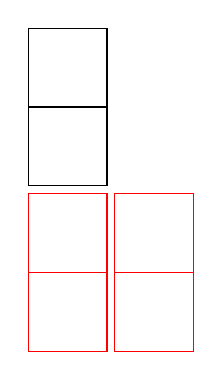
\begin{tikzpicture}
    \draw[draw=red] (0,0) rectangle ++(1,1);
    \draw[draw=red] (1.1,0) rectangle ++(1,1);
    \draw[draw=red] (0,1) rectangle ++(1,1);
    \draw[draw=red] (1.1,1) rectangle ++(1,1);
    \draw[draw=black] (0,2.1) rectangle ++(1,1);
    \draw[draw=black] (0,3.1) rectangle ++(1,1);
    \end{tikzpicture}
    \hspace{1cm}
    \begin{tikzpicture}
    \draw[draw=red] (0,0) rectangle ++(1,1);
    \draw[draw=red] (1.1,0) rectangle ++(1,1);
    \draw[draw=black] (1.1,1.1) rectangle ++(1,1);
    \draw[draw=black] (1.1,2.1) rectangle ++(1,1);
    \draw[draw=black] (1.1,3.1) rectangle ++(1,1);
    \end{tikzpicture}
    \hspace{1cm}
    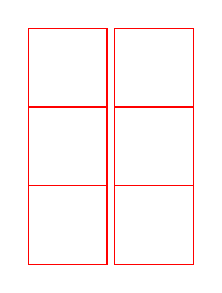
\begin{tikzpicture}
    \draw[draw=red] (0,0) rectangle ++(1,1);
    \draw[draw=red] (1.1,0) rectangle ++(1,1);
    \draw[draw=red] (0,1) rectangle ++(1,1);
    \draw[draw=red] (1.1,1) rectangle ++(1,1);
    \draw[draw=red] (0,2) rectangle ++(1,1);
    \draw[draw=red] (1.1,2) rectangle ++(1,1);
    \end{tikzpicture}

    \caption{Wizualizacja działania funkcji normalizującej dla liczb całkowitych (odpowiednio -2, 3 i 0), na czerwono zaznaczone są elementy które zostaną usunięte przez działanie tej funkcji.}
    \label{fig:int_norm}
\end{figure}
\subsection{Indukcyjny typ liczb całkowitych z jednoznaczną reprezentacją}
Mając już do dyspozycji funkcję normalizującą możemy wykorzystać idę jej działania do stworzenia typu indukcyjnego, który będzie charakteryzował się jednoznacznością reprezentacji. Sam ślad funkcji nie jest szczególnie ciekawy w tym przypadku. Możemy jednak dużo nauczyć się z ostatniego kroku procesu normalizacji. W kodzie \ref{int_norm} jest on uproszczony do \mintinline{coq}{_, _}, jednak pod tym wzorcem możemy wyróżnić trzy przypadki:
\begin{description}
    \item[\mintinline{coq}{S x', O}] - gdy wynikiem jest liczba ujemna o wartości \mintinline{coq}{S x'},
    \item[\mintinline{coq}{O, S y'}] - gdy wynikiem jest liczba dodatnia o wartości \mintinline{coq}{S y'},
    \item[\mintinline{coq}{O, O}] - gdy wynikiem jest zero.
\end{description}

Możemy zatem stworzyć typ indukcyjny z konstruktorami dla każdego z tych trzech przypadków.
\begin{code}
\begin{minted}{coq}
Inductive Z : Type :=
| Pos  : nat -> Z
| Zero : Z
| Neg  : nat -> Z.
\end{minted}
\caption{Definicja typu liczb całkowitych z jednoznaczną reprezentacją w Coqu.}
\label{Z}
\end{code}

Możemy w bardzo łatwy sposób zmodyfikować funkcję normalizującą \ref{int_norm}, na taką, która przekształca naszą naiwną reprezentację na nową, jednoznaczną. 
\begin{code}
\begin{minted}{coq}
Function int_to_Z (x y : nat) : Z :=
match x, y with
| S x', S y' => norm x' y'
| S x', O    => Neg x'
| O   , S y' => Pos y'
| O   , O    => Zero
end.
\end{minted}
\caption{Definicja funkcji przekształcającej naiwną reprezentację w jednoznaczną Coqu.}
\label{int_to_Z}
\end{code}

Taka definicja nie pozostawia wątpliwości co do swojej jednoznaczności, o ile oczywiście funkcja normalizująca jest poprawna. 
\subsection{Podstawowe operacje na jednoznacznych liczbach całkowitych}
Możemy teraz przejść do zdefiniowania kilku przykładowych funkcji dla liczb całkowitych, na zdefiniowanym powyżej typie \mintinline{coq}{Z} \ref{Z}. Tak jak w przypadku liczb naturalnych warto zacząć od rozpocząć od zdefiniowania następnika, a z racji posiadania liczb ujemnych również poprzednika.
\begin{code}
\begin{minted}{coq}
Definition succ (n: Z) : Z :=
match n with
| Pos k => Pos (S k)
| Zero => Pos O
| Neg O => Zero
| Neg (S n) => Neg n
end.
\end{minted}
\caption{Definicja następnika dla liczb całkowitych \mintinline{coq}{Z} \ref{Z}.}
\label{Z_succ}
\end{code}

\begin{code}
\begin{minted}{coq}
Definition pred (n: Z) : Z :=
match n with
| Pos (S n) => Pos n
| Pos O => Zero
| Zero => Neg O
| Neg n => Neg (S n)
end.
\end{minted}
\caption{Definicja poprzednika dla liczb całkowitych \mintinline{coq}{Z} \ref{Z}.}
\label{Z_pred}
\end{code}

\begin{code}
\begin{minted}{coq}
Definition neg (n: Z) : Z :=
match n with
| Pos k => Neg k
| Zero => Zero
| Neg k => Pos k
end.
\end{minted}
\caption{Definicja poprzednika dla liczb całkowitych \mintinline{coq}{Z} \ref{Z}.}
\label{Z_neg}
\end{code}
W obu przypadkach definicja jest dojść prosta i nie pozostawia za dużo wątpliwości co do swojej poprawności. W obu przypadkach konieczny był specjalny 4 przypadek, który odpowiada za przejście do zero. Definicja negacji jest wyjątkowo trywialna w przypadku tej reprezentacji, więc nie wymaga omówienia. Przejdziemy zatem to najważniejszej operacji na liczbach całkowitych, jaką jest dodawanie.
\begin{code}
\begin{minted}{coq}
Fixpoint map_n {A: Type} (n: nat) (f: A -> A) (x: A) : A :=
match n with
| O    => x
| S n' => f (map_n n' f x)
end.

Definition add (a b : Z) : Z :=
match a with 
| Pos n => map_n (S n) succ b
| Zero  => b
| Neg n => map_n (S n) pred b
end.
\end{minted}
\caption{Definicja dodawania dla liczb całkowitych \mintinline{coq}{Z} \ref{Z}.}
\label{Z_add}
\end{code}

W przedstawionej w tej pracy definicji dodawania \ref{Z_add} została wykorzystana funkcja pomocnicza \mintinline{coq}{map_n} \ref{Z_add}. Pozwala ona na nałożenie $n$ operacji na daną wartość. Z uwagi iż nasze liczby całkowite wykorzystują liczby naturalne oczywistym jest zdefiniowanie dodawania jako wykonanie $n$ operacji następnika, lub poprzednika jeśli liczba którą dodajemy była ujemna. Odejmowanie można w łatwy sposób zdefiować jako dodawane liczby przeciwnej. Możemy zatem zdefiniować ostania, lecz równie ważną operację mnożenia.
\begin{code}
\begin{minted}{coq}

Definition mul (a b: Z) : Z :=
match a with 
| Pos n => map_n (S n) (add b) Zero
| Zero  => Zero
| Neg n => neg (map_n (S n) (add b) Zero)
end.
\end{minted}
\caption{Definicja mnożenia dla liczb całkowitych \mintinline{coq}{Z} \ref{Z}.}
\label{Z_mul}
\end{code}

Definicja mnożenia wykorzystuje podobny mechanizm jak dodawanie, z tą różnicą, że tym razem nie dodajemy jedynki od wyniku, a całą liczbę przez którą mnożymy. Jest to dojść znana rekurencyjna definicja mnożenia, więc nie będziemy poświęcać zbyt dużo czasu na nią. Wszystkie przedstawione powyżej operacji i nie tylko, wraz z dowodami ich podstawowymi prawami, takimi jak łączność, przemienność, oraz rozdzielność mnożenia względem dodawania można znaleźć w dodatku better\_integer.v.
\section{Egzotyczne liczby całkowite}
Poprzednia definicja liczb całkowitych wydaje się być naturalnym kandydatem, z uwagi na powiązanie z funkcją normalizującą, a dodatkowo pozwala na łatwe obliczenia. Większość konkurencyjnych definicji jest bardzo podobna, czasami zamiast symetrycznych trzech konstruktorów wykorzystują one dwa i jeden z nich jest obciążony zerem. Niesmak może jednak pozostawiać fakt, iż wykorzystują one w swojej definicji liczby naturalne. Nasuwa się zatem pytanie czy można zdefiniować liczby całkowite bez odwoływania się do liczb naturalnych?
\subsection{Inne spojrzenie na normalizację}
W poprzedniej sekcji patrzyliśmy na proces normalizacji "od dołu do góry", który polegał na usuwaniu następników z obu elementów pary, aż jedna będzie zerem. Możemy jednak odwrócić ten proces tworząc pewien proces pseudo-normalizacji, skupiając się na spojrzeniu "od góry do dołu". W tym procesie będziemy zliczać ile elementów jest powyżej, nie wiedząc jednak czy zliczamy następnik, czy poprzedniki. Dopiero po osiągnięciu punktu, w którym obie wartości są takie same, będziemy w stanie zweryfikować, czy liczba jest dodatnia czy ujemna. 
\begin{figure}[!htp]
    \centering

    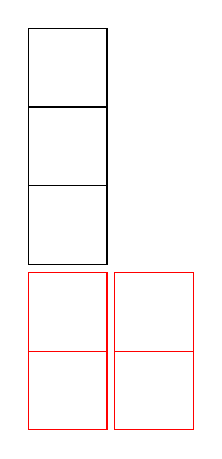
\begin{tikzpicture}
    \draw[draw=red] (0,0) rectangle ++(1,1);
    \draw[draw=red] (1.1,0) rectangle ++(1,1);
    \draw[draw=red] (0,1) rectangle ++(1,1);
    \draw[draw=red] (1.1,1) rectangle ++(1,1);
    \draw[draw=black] (0,2.1) rectangle ++(1,1);
    \draw[draw=black] (0,3.1) rectangle ++(1,1);
    \draw[draw=black] (0,4.1) rectangle ++(1,1);
    \end{tikzpicture}
    \hspace{1cm}
    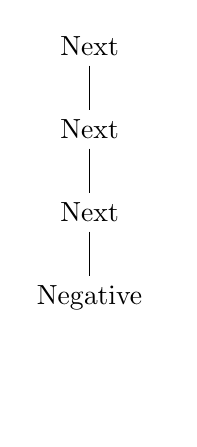
\begin{tikzpicture}[grow'=down]
    \tikzset{level distance=30pt}
    \Tree [.Next [.Next [.Next Negative ] ] ]
    \draw[draw=white] (0,-4.6) rectangle ++(1,1);
    \end{tikzpicture}

    \caption{Wizualizacja działania pseudo-normalizacji "od góry do dołu".}
    \label{fig:int_psudonorm}
\end{figure}
\subsection{Następniko-poprzednik jako ślad pseudo-normalizacji}
Możemy teraz stworzyć typ iniektywny bazujący na śladzie zaprezentowanej pseudo-normalizacji. Żeby jednak był on jednoznaczny poprzebujemy pozbyć się problemu zera. W zaprezentowanej powyżej intuicji nie wiadomo w jaki sposób powinno być one reprezentowane, gdyż sytuacja w której zaczynamy od równych wartości żadna wartość nie jest większa, a więc nie wiadomo którego konstruktora użyć. Ten problem rozwiążemy zaburzając symetrię między konstruktorami. Jeden z nich będzie reprezentować zero, i w jego kontekście \mintinline{coq}{Next} będzie następnikiem, a więc \mintinline{coq}{Next Zero} będzie reprezentować jedynkę. Drugi natomiast będzie minus jedynką, a \mintinline{coq}{Next} zaaplikowany na nim będzie oznaczać poprzednik.

\begin{code}
\begin{minted}{coq}
Inductive Z' : Type :=
| Zero     : Z'
| MinusOne : Z'
| Next     : Z' -> Z'.
\end{minted}
\caption{Definicja liczby całkowitych z następniko-poprzednikiem.}
\label{Z'}
\end{code}
\subsection{Operacje na liczbach z następniko-poprzednikiem}
Konstrukcja liczb z następniko-poprzednikiem pozwala na jednoznaczną reprezentację, nie jest jednak zbyt wygodna do przeprowadzania obliczeń. Podstawowe operacje takie jak następnik, czy poprzednik mają liniową złożoność obliczeniową względem wielkości liczby. Wszystko za sprawą faktu, że aby wiedzieć czy powinniśmy dodać następniko-poprzednik czy go usunąć musimy wiedzieć czym on tak naprawdę jest, a więc musimy sprawdzić ostatni konstruktor.
\begin{code}
\begin{minted}{coq}
Function succ (k : Z') : Z' :=
match k with
| Zero => Next Zero
| MinusOne => Zero
| Next Zero => Next (Next Zero)
| Next MinusOne => MinusOne
| Next k' => Next (succ k')
end.
\end{minted}
\caption{Definicja następnika liczb całkowitych z następniko-poprzednikiem \ref{Z'}.}
\label{Z'_succ}
\end{code}
\begin{code}
\begin{minted}{coq}
Function pred (k : Z') : Z' :=
match k with
| Zero => MinusOne
| MinusOne => Next MinusOne
| Next Zero => Zero
| Next MinusOne => Next (Next MinusOne)
| Next k' => Next (pred k')
end.
\end{minted}
\caption{Definicja poprzednika liczb całkowitych z następniko-poprzednikiem \ref{Z'}.}
\label{Z'_pred}
\end{code}

Oczywiście bardziej zaawansowane operacje jak dodawanie czy mnożenie można zdefiniować, lecz definicje te nie są szczególnie przyjemne. Pominiemy je zatem w tej pracy. Definicję dodawania wraz z dowodem na izomorfizm pomiędzy tą definicją liczb całkowitych, a tą nieco bardziej klasyczną zaprezentowaną w poprzedniej sekcji możemy znaleźć w dodatku integer\_izo.v.
\section{Dodatnie liczby wymierne}
W przeciwieństwie do liczb całkowitych znalezienie jednoznacznej reprezentacji dla liczb wymiernych nie jest prostym zadanie. Ta sekcja jest operta na pracy Yves Bertot'a \cite{Qplus} w której przedstawił koncept reprezentowania liczb wymiernych za pomocą śladu algorytmu Euklidesa.
\subsection{Normalizacja liczb wymiernych}
Korzystając z podstawowej wiedzy na temat ułamków wiemy, że istnieje nieskończenie wiele reprezentacji tego samego ułamka. Zapisy takie jak $\frac{1}{2}$, $\frac{2}{4}$, czy $\frac{50}{25}$ wyrażają taką samą wartość: pół. Za postać normalną z reguły uznaje taką formę, w której nie można dokonać już operacji skrócenia ułamka, czyli podzielenia jego licznika i mianownika przez tą samą liczbę. Aby poznać przez jaką liczbę należy podzielić obie strony ułamka, aby uzyskać postać nieskracalną należy wyliczyć największy wspólny dzielnik. Jednym ze sposobów na jego wyznaczenie, jest właśnie postępowanie zgodnie z algorytmem Euklidesa \ref{euclid}. 
\begin{code}
\begin{minted}{coq}
Function euclid (p q: nat) : nat :=
match compare p q with
| Eq => p
| Gt => euclid (p - q) q n'
| Lt => euclid p (q - p) n'
end.
\end{minted}
\caption{Definicja klasycznego algorytmu Euklidesa w pseudo Coqu.}
\label{euclid}
\end{code}
Algorytm ten bazuje na prawie $\textrm{NWD}(a, b) = \textrm{NWD}(a - b, b)$, jeśli $a > b$. Inną ciekawą obserwacją z której skorzystamy, jest to że ślad algorytmu nie zmieni się, jeśli przemnożymy obie liczby przez dowolną dodatnią liczbę naturalną, w przykładzie poniżej $k$.

\begin{equation}
    \begin{split}
        11k&>5k\\
        (11-5)k=6k&>5k\\
        (6-5)k=k&<4k\\
        k&<3k=(4-1)k\\
        k&<2k=(3-1)k\\
        k&=k=(2-1)k
    \end{split}
\end{equation}

Jak widzimy w przykładzie powyżej ślad, czyli to która liczba okazała się większa nie zależy od wybranego $k$. Jedyne co się zmieniło to wyliczony największy wspólny dzielnik został przemnożony przez stałą $k$. Dodatkowo znając ślad możemy odtworzyć argumenty, z dokładnością do największego wspólnego dzielnika. Możemy zatem użyć tych śladów do jednoznacznego reprezentowania liczb wymiernych. Dowód tego faktu, jak i innych związanych z śladami algorytmów Euklidesa możemy znaleźć w dodatku Qplus.v. 
\subsection{Typ liczb wymiernych dodatnich}
Zdefiniujmy zatem typ śladów algorytmu Euklidesa \ref{Qplus}.
\begin{code}
\begin{minted}{coq}
Inductive Qplus : Type :=
| One : Qplus
| N   : Qplus -> Qplus
| D   : Qplus -> Qplus.
\end{minted}
\caption{Definicja typu śladów algorytmu Euklidesa w Coqu.}
\label{Qplus}
\end{code}
Jak mogliśmy się spodziewać składa się on z trzech konstruktorów: \mintinline{coq}{N} kiedy licznik jest większy od mianowania, \mintinline{coq}{D} gdy mianownik jest większy, oraz \mintinline{coq}{One} gdy obie wartości były równe, co zakończyło proces normalizacji. Taka konstrukcja dodatkowo zapewnia nam przyjazną indukcję po wszystkich dodatnich liczbach wymiernych, w przeciwieństwie do naiwnej reprezentacji \ref{Q} wykorzystującej parę liczb naturalnych.
\begin{code}
\begin{minted}{coq}
Definition Q : Type := (nat * nat).
\end{minted}
\caption{Definicja naiwnej reprezentacji liczb wymiernych w Coqu.}
\label{Q}
\end{code}
\subsection{Funkcje przejścia między reprezentacjami}
Wiedząc że \mintinline{coq}{Qplus} \ref{Qplus} reprezentuje ślady algorytmu Euklidesa powinniśmy być w stanie w miarę łatwo napisać kod funkcji go generującej. Niestety rzeczywistość Coqa jest dojść brutalna i termination checker nie potrafi wyznaczyć dobrze ufundowanego porządku na argumentach algorytmu Euklidesa. My wiemy że jest nim suma argumentów, lecz przekracza to jego automatyczne możliwości. Posłużymy się zatem konceptem zwanym paliwem. Polega on na dodaniu dodatkowego parametru funkcji, który będzie się zmniejszał z każdym wywołaniem rekurencyjnym funkcji, gwarantując terminację w oczach Coqa. Ustalając wartość tego parametru dostatecznie wysoko, będziemy mogli wyliczyć ślad zanim skończy nam się paliwo.
\begin{code}
\begin{minted}{coq}
Function qplus_c' (p q n: nat) : Qplus :=
match n with
| O    => One
| S n' => match compare p q with
          | Eq => One
          | Gt => N (qplus_c' (p - q) q n')
          | Lt => D (qplus_c' p (q - p) n')
          end
end.

Function qplus_c (x: Q) : Qplus :=
  let (p, q) := x in qplus_c' p q ((p + q) / gcd p q).
\end{minted}
\caption{Definicja funkcji przekształcającą naiwną reprezentację w ilorazowy typ dodanych liczb wymiernych w Coqu.}
\label{qplus_c}
\end{code}

Jak widzimy w definicji funkcji \ref{qplus_c} paliwo zostało ustalone jako suma argumentów podzielona przez ich największy wspólny dzielnik. Wiemy, że w każdej iteracji algorytm Euklidesa zmniejsza sumę argumentów przynajmniej o ich największy wspólny dzielnik, mamy zatem pewność że zdążymy wyliczyć cały ślad tego algorytmu.

Funkcja odwrotna (z dokładnością do NWD) do zaprezentowanej powyżej ma równie oczywistą konstrukcję. Będziemy odwracać proces poprzez dodawanie wartości drugiego argumentu do tego który w trakcie normalizacji był większy. Wynika to z dojść oczywistego faktu, że $(p - q) + q = p$.
\begin{code}
\begin{minted}{coq}
Function qplus_i (x : Qplus) : Q :=
match x with
| One  => (1, 1)
| N x' => let (p, q) := qplus_i x' in (p + q, q)
| D x' => let (p, q) := qplus_i x' in (p, p + q)
end.
\end{minted}
\caption{Definicja funkcji przekształcającą ilorazowy typ dodanych liczb wymiernych do naiwnej reprezentacji w Coqu.}
\label{qplus_c}
\end{code}
\subsection{Rozszerzenie do ciała liczb wymiernych}
Same dodatnie liczby wymierne nie są aż tak użyteczne jak całe ciało liczb wymiernych. Na szczęście istnieje prosty sposób na rozszerzenie tego konceptu, do wszystkich liczb wymiernych. Skorzystamy tutaj z konstrukcji podobnej do tej zaprezentowanej przy liczbach, a więc dodamy typ z trzema konstruktorami: dla liczb dodatnich, dla ujemnych oraz dla zera.
\begin{code}
\begin{minted}{coq}
Inductive FullQ :=
| Pos  : Qplus -> FullQ
| Zero : FullQ
| Neg  : Qplus -> FullQ.
\end{minted}
\caption{Definicja ilorazowego typu liczb wymiernych w Coqu.}
\label{FullQ}
\end{code}
\subsection{Operacje na liczbach wymiernych}
TODO


\section{Wolne grupy}
W tym rozdziale poznaliśmy już wolne monoidy, teraz przyszedł czas na ich bardziej skomplikowaną wersję, czyli grupy. Ma ona trzy podstawowe prawa: istnienie elementu neutralnego, łączność działania oraz istnienie elementu przeciwnego.
\begin{description}
\item[Element neutralny:] $\exists e \in \mathbf{A}, \forall x \in \mathbf{A}, e \circ x = x = x \circ e$
\item[Łączność działania:] $\forall x y z \in \mathbf{A}, x \circ (y \circ z) = (x \circ y) \circ z$
\item[Element odwrotny:] $\forall x \in \mathbf{A}, \exists x^{-1} \in \mathbf{A}, x \circ x^{-1} = x^{-1} \circ x = e$
\end{description}
Jak więc możemy zaobserwować każda grupa jest również monoidem, a jedyne co się zmienia to nowa operacja odwrotności. Jak więc możemy się domyślać wolną grupą będą listy z elementami oraz ich odwrotnościami. Naiwną implementację możemy zatem zapisać jako listę par elementu z boolem, który będzie przechowywać informację czy to ten element czy element do niego odwrotny.  
\begin{code}
\begin{minted}{coq}
Definition CanonFreeGroup (A: Type) := list (bool*A).
\end{minted}
\caption{Naiwna implementacja wolnej grupy w Coqu.}
\label{CanonFreeGroup}
\end{code}
\subsection{Normalizacja wolnej grupy}
Od normalizowanej wolnej grupy będziemy wymagać, aby dwa wzajemnie odwrotne elementy nie były swoimi sąsiadami, gdyż jak wiemy z praw grupy takie elementy się "anihilują" i są równoważne elementowi neutralnemu. 
\begin{code}
\begin{minted}{coq}
Inductive Normalized {A: Type} `{Group A} : CanonFreeGroup A -> Prop :=
| NNil   : Normalized []
| NSingl : forall (b : bool) (v : A), Normalized [(b, v)]
| NCons  : forall (b b': bool) (v v' : A) (x: CanonFreeGroup A), 
            v <> v' \/ b = b' -> Normalized ((b', v') :: x) ->
            Normalized ((b, v) :: (b', v') :: x).
\end{minted}
\caption{Predykat bycia w postaci normalnej dla wolnej grupy w Coqu.}
\label{Normalized}
\end{code}
Predykat bycia w postaci normalnej możemy wyrazić za pomocą typu induktywnego z trzema konstruktorami dla pustej grupy, singletona, oraz dla następnika \ref{Normalized}. Funkcję normalizującą\ref{normalize} również bez większych problemów da się wyrazić, jednak, żeby to zrobić nasz typ bazowy będzie musiał posiadać zdefiniowaną rozstrzygalną równość na naszym typie bazowym, w postaci funkcji \mintinline{coq}{eqf}.
\begin{code}
\begin{minted}{coq}
Class Group (A : Type) := GroupDef {
  zero      : A;
  op        : A -> A -> A;
  inv       : A -> A;
  eqf       : A -> A -> bool;
  left_id   : forall x: A, op zero x = x;
  right_id  : forall x: A, op x zero = x;
  left_inv  : forall x: A, op (inv x) x = zero;
  right_inv : forall x: A, op x (inv x) = zero;
  op_assoc  : forall x y z: A, op (op x y) z = op x (op y z);
  eqf_eq    : forall x y, reflect (x = y) (eqf x y)
}.
\end{minted}
\caption{Klasa grup z rozstrzygalną równością w Coqu.}
\label{normalize}
\end{code}

\begin{code}
\begin{minted}{coq}
Fixpoint normalize {A: Type} `{Group A} (x: CanonFreeGroup A) :=
match x with
| [] => []
| (b, v) :: x' => 
    match normalize x' with
    | [] => [(b, v)]
    | (b', v') :: x'' => if andb (eqf v v') (xorb b b')
                         then x''
                         else (b, v) :: (b', v') :: x''
    end
end.
\end{minted}
\caption{Funkcja normalizująca wolną grupą w Coqu.}
\label{normalize}
\end{code}
\subsection{Jednoznaczny typ dla wolnych grup w Coqu}
Wiedząc już czym charakteryzują się wolne grupy znormalizowane, możemy przejść do stworzenia typu induktywnego dla nich bazując na funkcji normalizacji. Pierwszą ważną obserwacją jest to, że funkcja zaczyna swoją normalizację od końca, wyznaczając element początkowy. Pod drugie wyrażenie \mintinline{coq}{eqf v v'} jest równoważne przyrównaniu do elementu neutralnego, różnicy  \mintinline{coq}{v} oraz \mintinline{coq}{v'}, czyli \mintinline{coq}{eqf (op v (inv v')) zero}. A więc tak naprawdę interesują nasz różnice między elementami. Po trzecie podobnie jak w przypadku elementów, tu również interesują nasz różnice między kolejnymi znakami. Nasz typ ilorazowy będzie zatem odwrotną listą różnicową elementów i ich znaków, czyli taką w której różnice odnoszą się do poprzedniego elementu, z dodatkowym warunkiem zabezpieczającym przed postawieniem dwóch tych samych elementów z innym znakiem obok siebie.
\begin{code}
\begin{minted}{coq}
Inductive NonEmptyFreeGroup (A: Type) `{Group A} :=
| Singl  : bool -> A -> NonEmptyFreeGroup A
| Switch : forall x: A, Squash (x <> zero) -> NonEmptyFreeGroup A -> NonEmptyFreeGroup A
| Stay   : A -> NonEmptyFreeGroup A -> NonEmptyFreeGroup A.

Definition FreeGroup (A: Type) `{Group A} := option (NonEmptyFreeGroup A).
\end{minted}
\caption{Ilorazowy typ wolnej grupy w Coqu.}
\label{FreeGroup}
\end{code}

Jak widzimy w definicji \ref{FreeGroup} mamy tak naprawdę dwa typy, pustych oraz nie pustych list wolnych. Wynika to z problemu niejednoznaczności dla elementu neutralnego (pustej grupy). Odwrotnością elementu neutralnego jest on sam, a więc zgodnie z prawami nie powinna istnieć pusta grupa "dodatnia" oraz "ujemna", stąd też potrzeba zdefiniowania niepustej wolnej grupy. Sama jej definicja składa się z trzech konstruktorów. Singleton jest dojść prostym konstruktorem bez niespodzianek. Drugi konstruktor natomiast reprezentuje zmianę znaku w stosunku do poprzedniego elementu, w związku z tym wymaga on aby różnica elementów była różna od 0, gdyż w przeciwnym wypadku obok siebie stałyby te same elementy z przeciwnymi znakami. Żeby nie martwić się o jednoznaczność dowodu został on opakowany w \mintinline{coq}{Squash} a więc żyje w świecie z definicyjną irrelewancją dowodów. Ostatni z konstruktorów reprezentuje różnicę bez zmiany znaków, w takim wypadku nie są potrzebne dodatkowe dowody, a więc jest on dojść prosty. Niestety, wymaganie odnośnie wyliczania różnicy wymusza, aby typ bazowy był sam w sobie grupą z operacją odwrotności.
\subsection{Funkcje przejścia między reprezentacjami}
Mając już zdefiniowany typ ilorazowy dla wolnych list powinniśmy zdefiniować funkcję która pozwoli nam przekonwertować naszą nawianą reprezentację do typu ilorazowego. Jej definicja nie jest zupełnie trywialne ze względu na zastosowany typ zależny w drugim konstruktorze.
\begin{code}
\begin{minted}{coq}
Fixpoint to_uniq' {A: Type} `{Group A} (b : bool) (v: A) (x: CanonFreeGroup A) 
: NonEmptyFreeGroup A :=
match x with 
| []             => Singl b v
| (b', v') :: x' => 
    if eqb b b' 
    then Stay (sub v v') (to_uniq' b' v' x')
    else match eqf_eq (sub v v') zero with
         | ReflectF _ p => Switch (sub v v') (squash p) (to_uniq' b' v' x')
         | _  => (Singl b v) (* invalid *)
         end
end.

Definition to_uniq {A: Type} `{Group A} (x: CanonFreeGroup A) : FreeGroup A :=
match x with
| [] => None
| (b, v) :: x' => Some (to_uniq' b v x')
end.
\end{minted}
\caption{Definicja funkcji przekształcającej naiwną reprezentacje w ilorazową w Coqu.}
\label{to_uniq}
\end{code}

Jak widzimy w definicji funkcji \mintinline{coq}{to_uniq} \ref{to_uniq}, w przypadku w którym zmieniamy znak musimy wyciągnąć dowód, że dwa kolejne elementy są od siebie różne. Na szczęście użycie \mintinline{coq}{reflect} w definicji grupy pozwala nam w łatwy sposób wyciągnąć taki dowód, jeśli funkcja \mintinline{coq}{eqf} zwraca \mintinline{coq}{false}. W przeciwnym zaś przypadku funkcja zwraca cokolwiek. Wprawne oko pozwala wypatrzeć, że funkcja \mintinline{coq}{to_uniq} działa poprawnie tylko dla znormalizowanych wolnych grup, jeśli chcemy pozbyć się tego ograniczenia należy ją złożyć z funkcją normalizującą \mintinline{coq}{normalize} \ref{normalize}.

\begin{code}
\begin{minted}{coq}
Fixpoint to_canon' {A: Type} `{Group A} (x: NonEmptyFreeGroup A) : CanonFreeGroup A :=
match x with 
| Singl b v     => [(b, v)]
| Stay v x'     => match to_canon' x' with
                   | [] => [(true, v)] (* invalid *)
                   | (b, v') :: y => (b, op v v') :: (b, v') :: y
                   end
| Switch v _ x' => match to_canon' x' with
                   | [] => [(true, v)] (* invalid *)
                   | (b, v') :: y => (negb b, op v v') :: (b, v') :: y
                   end
end.

Definition to_canon {A: Type} `{Group A} (x: FreeGroup A) : CanonFreeGroup A :=
match x with
| None => []
| Some x' => to_canon' x'
end.
\end{minted}
\caption{Definicja funkcji przekształcającej ilorazową reprezentacje w naiwną w Coqu.}
\label{to_canon}
\end{code}

Funkcja odwrotna \mintinline{coq}{to_canon} \ref{to_canon} ma nieco prostszy kod, gdyż nie wymaga ona tworzenia typów zależnych. Cała jej idea skupia się dodawania zapisanej różnicy do poprzedniego elementu i dzięki temu wyliczanie kolejnych wartości wolnej grupy.
\subsection{Wolna grupa jako grupa}

\subsection{Wolna grupa jako monada}
\subsection{Zastosowania wolnych grup}
\section{Listy różnicowe jak multi-zbiory}
W poprzednim rozdziale pokazaliśmy jak można zdefiniować zbiry i multi-zbiory w Coqu używając pod-typowania. Jest to skuteczna strategia, której niestety nie da się przenieść do języków nie posiadających typów zależnych takich jak Haskell. Nasuwa się zatem pytanie czy istnieją typy bazowe dla których można zdefiniować multi-zbiory bez wykorzystania pod-typowania. W tym celu wykorzystamy listę różnic pomiędzy kolejnymi elementami multi-zbioru.
\subsection{Funkcja normalizująca}
Jak można się domyślać w celu normalizacji listy elementów w multi-zbiór posłużymy się funkcją sortującą, podobnie jak w poprzednim rozdziale. 
\begin{code}
\begin{minted}{coq}
Fixpoint min (h: nat) (l: list nat) : nat :=
match l with
| [] => h
| (h' :: l') => if h' <=? h then min h' l' else min h l'
end.

Fixpoint sub_list (s: nat) (l: list nat) : list nat :=
match l with
| [] => []
| (h :: l') => (h - s) :: sub_list s l'
end.

Fixpoint rm_one_zero (l: list nat) : list nat :=
match l with
| [] => []
| (h :: l') => if h =? O then l' else h :: rm_one_zero l'
end.

Fixpoint select_sort' (f: nat) (prev: nat) (l : list nat) : list nat :=
match f with
| O => []
| S f' =>
  match l with
  | [] => []
  | (h :: l') => let m := min h l' in
                 let p := prev + m in
                 p :: (select_sort' f' p (rm_one_zero (sub_list m l)))
  end
end.

Definition select_sort (l : list nat) : list nat :=
  select_sort' (length l) O l.
\end{minted}
\caption{Definicja sortowania przez wybieranie dla liczb naturalnych w Coqu.}
\label{select_sort}
\end{code}
Tutaj w jednak przyjrzymy się pewnemu zmodyfikowanemu algorytmowi sortowanie przez wybieranie dla liczb naturalnych \ref{select_sort}. Modyfikacja ta polega na zoptymalizowaniu kolejnych operacji porównań poprzez odjęcie od każdej liczby znalezione minimum. Porównywanie liczb naturalnych w systemie unarnym jest liniowe względem mniejszej z liczb, w związku z tym im mniejsze liczby na liście tym szybszy proces szukania minimum. Możemy się teraz przyjrzeć śladowi tej funkcji, a konkretnie jak będą wyglądać kolejne minima na sortowanej liście. Z uwagi na to iż w każdym wywołaniu rekurencyjnym wartości są pomniejszane o minimum to kolejne wyliczane minima będą stanowić różnicę pomiędzy kolejnymi (zgodnie z porządkiem na liczbach naturalnych) elementami.
\subsection{Typ ilorazowy dla multi-zbiorów}
Zanim przystąpimy do implementacji typu ilorazowego postaramy się uogólnić przedstawiony powyżej schemat na więcej typów. Po pierwsze potrzebujemy, aby na typie istniał porządek liniowy, gdyż istniały dwie różne minimalne wartości nie moglibyśmy zawsze wyznaczyć unikalnego minimum. Po drugie musi istnieć jakaś operacja różnicy dwóch elementów, oraz operacja dodawania różnicy do wartości, aby odzyskać oryginalny multi-zbiór.
\begin{code}
\begin{minted}{coq}
Class Diff (A: Type) `{E: EqDec A} := {
  D: Type;
  diff: A -> A -> D;
  add: A -> D -> A;

  diff_comm: forall x y, diff x y = diff y x;
  diff_def: forall x d, d = diff x (add x d);
  recover: forall x y, y = add x (diff x y) \/ x = add y (diff x y);
  diff_anti_sym : forall x d, x = add (add x d) d -> d = diff x x;
  diff_trans: forall x y z, 
    z = add (add x (diff x y)) (diff y z) -> z = add x (diff x z);
}.
\end{minted}
\caption{Definicja klasy typów dla której istnieją unikatowe listy różnicowe w Coqu.}
\label{Diff}
\end{code}
W tej pracy została ostatecznie wykorzystana definicja\ref{Diff} w która swoją konstrukcją implikuje istnienie porządku liniowego, w związku z tym nie wymaga ona jego istnienia jako przesłanki. Wymaga ona za to istnienie typu różnic symetrycznych, funkcji która dla dwóch elementów wylicza takową różnicę oraz funkcja dodająca wskazaną różnicę do elementu. Dodatkowo będziemy wymagać spełnienia pięciu praw. Po pierwsze wymusza symetryczność różnicy, poprzez wymaganie przemienności operacji. Drugie definiuje związek pomiędzy operacją różnicy symetrycznej a dodawaniem. Trzecie prawo wymaga aby z różnicy symetrycznej dało się odzyskać przynajmniej jeden z elementów. Czwarte mówi o tym, że jeśli dwa razy dodaliśmy jakąś różnicę i wynik się nie zmienił to znaczy że ta różnica jest neutralna, prawo to wraz z trzecim implikuje anty-symetryczność generowanego porządku. Piąte prawo wymaga aby nasze różnice symetryczne były przechodnie, a więc jeśli da się odzyskać jakąś wartość dodając dwie różnice o wspólnym końcu to można ją odzyskać z bezpośredniej różnicy. Mając te prawa możemy zdefiniować porządek liniowy, dwa elementy będą z sobą w relacji wtedy i tylko wtedy gdy dodanie do pierwszej ich wspólnej różnicy daje nam drugą. W dodatku $DifferentialLists.v$ znajduje się dowód tego faktu. Mając zdefiniowana klasę możemy napisać typ list różnicowych\ref{DiffList}.
\begin{code}
\begin{minted}{coq}
Definition DiffList (A: Type) `{Diff A} :=
  option (A * list D).
\end{minted}
\caption{Definicja list różnicowych w Coqu.}
\label{DiffList}
\end{code}
Typ ten jest zdefiniowany za pomocą opcji, która umożliwia istnienie pustych multi-zbiorów. W środku opcji mamy głowę listy typu bazowego, wraz z listą różnic.
\subsection{Funkcje przejścia między reprezentacjami}
Po zdefiniowaniu kształtu typu multi-zbiorów z wykorzystaniem list różnicowych, możemy napisać funkcję które pozwolą na przejście między reprezentacją listową a ilorazową.
\begin{code}
\begin{minted}{coq}
Fixpoint from_diff' {A: Type} `{Diff A} (x: A) (l: list D) :=
  match l with
  | []        => [x]
  | (h :: l') => x :: from_diff' (add x h) l'
  end.

Definition from_diff {A: Type} `{Diff A} (x: DiffList A) : list A :=
  match x with
  | None        => []
  | Some (a, l) => (from_diff' a l)
  end.
\end{minted}
\caption{Definicja funkcji przejścia z listy różnicowej do listowej postaci multi_zbioru w Coqu.}
\label{from_diff}
\end{code}

Funkcja \mintinline{coq}{from_diff} \ref{from_diff} pozwana nam wygenerować listę elementów z listy różnic. Zasada działania jest bardzo prosta. Po pierwsze dla pustej listy różnicowej zwraca listę pustą. Dla listy różnicowej z samą głową zwracamy singleton. W przypadku dłuższych listy kolejne wartości będą stanowić sumy elementu poprzedzającego wraz z koleją różnicą.

\begin{code}
\begin{minted}{coq}
Fixpoint to_diff_sorted' {A: Type} `{Diff A} (p: A) (l: list A) : list D :=
  match l with
  | [] => []
  | (h :: t) => diff p h :: to_diff_sorted' h t
  end.

Definition to_diff_sorted {A: Type} `{Diff A} (l: list A) : DiffList A :=
  match l with
  | [] => None
  | (h :: t) => Some (h, to_diff_sorted' h t)
  end.

Definition to_diff {A: Type} `{Diff A} (l: list A) : DiffList A :=
  to_diff_sorted (mergeSort ord l).
\end{minted}
\caption{Definicja funkcji przejścia z listowej postaci multi-zbioru do listy różnicowej w Coqu.}
\label{to_diff}
\end{code}

Funkcja \mintinline{coq}{to_diff} \ref{from_diff} to złożenie dwóch funkcji: sortującej z funkcją generującą listy różnicowe. Zasada jej działania jest również bardzo prosta i polega na wyliczaniu kolejnych różnic pomiędzy elementami listy. Naturalnie pierwszy element listy zostaje zapisany jako głowa listy różnicowej. Obie te funkcje są dojść proste. Można udowodnić, że są one swoimi odwrotnościami z dokładnością do permutacji elementów. Dodatkowo można za ich pomocą potwierdzić, że nasz typ multi-zbioru jest rzeczywiście ilorazowy poprzez wykazanie, że jeśli dwie listy są swoimi permutacjami, to po przejściu do postaci list różnicowych ich reprezentacje będą sobie równe. Dowód tych dwóch faktów można znaleźć w dodatku $DifferentialLists.v$.
\subsection{Operacje na listach różnicowych}
Mając zdefiniowane funkcje przejścia między listami różnicowymi możemy w łatwy sposób wykorzystać wszystkie funkcje zaimplementowane dla list. Oznacza to że nasza implementacja jest zarówno funktorem jak i monadą, oczywiście przyjmując że typ wynikowy również implementuje klasę \mintinline{coq}{Diff} \ref{diff}. Przejście między reprezentacjami jest jednak kosztowne i ma liniową złożoność obliczeniową względem długości listy. Zatem operacje takie jak dodanie elementu lepiej jest zaimplementować bezpośrednio na liście różnicowej. Przyjrzyjmy się implementacji funkcji \ref{add_to_diff} dodającej $x$.
\begin{code}
\begin{minted}{coq}
Fixpoint add_to_diff' {A: Type} `{Diff A} (x: A) (h: A) (l: list D) : list D :=
match l with
| [] => [diff h x]
| (d :: l') => if ord x (add h d)
               then diff h x :: diff x (add h d) :: l'
               else d :: add_to_diff' x (add h d) l'
end.

Definition add_to_diff {A: Type} `{Diff A} (x: A) (l: DiffList A) : DiffList A :=
match l with
| None => Some (x, [])
| Some (h, l) => if ord x h
                 then Some (x, diff x h :: l)
                 else Some (h, add_to_diff' x h l)
end.
\end{minted}
\caption{Definicja funkcji dodającej element do listy różnicowej w Coqu.}
\label{add_to_diff}
\end{code}
Przechodzi ona przez listę aż do momentu napotkania pozycji na której znajduje się wartość od niej większa. Po jej napotkaniu tworzy dwie różnice pomiędzy poprzednim elementem a $x$ oraz pomiędzy $x$ a następnym elementem (czyli sumie poprzedniego i kolejnej różnicy na liście). Możemy udowodnić że po zaaplikowaniu takiej funkcji na liście znajduje się element $x$, żaden element nie został usunięty, oraz to że długość listy zwiększyła się o 1. Dowody tych faktów można znaleźć również w dodatku $DifferentialLists.v$.

    \chapter{Function types as quotient types}
	%W tym rozdziale zostanie przedstawione w jaki sposób możemy wykorzystać typ funkcji do zdefiniowania pewnych typów ilorazowych. Niestety przestawione poniżej przykłady tworzą więcej problemów niż rozwiązują, w związku z tym są praktycznie bezużyteczne w realnych aplikacjach, nie mniej jednak stanowią ciekawy przykład niekonwencjonalnego podejścia do problemu. Dlatego zostały zamieszczone w tym krótkim rozdziale.
\section{Jak funkcje utożsamiają elementy}
Na początku pracy wspomnieliśmy, iż nie można zdefiniować typu zbiorów oraz multi-zbiorów na dowolnego typu bazowego. Jest to prawda w przypadku typów induktywnych, w których kolejność konstruktorów ma znaczenie, możemy natomiast wykorzystać wbudowany w praktycznie każdy język programowania typ funkcji. Naturalnie, aby móc w rozsądny sposób rozumować o równościach na funkcjach będziemy musieli zapostulować aksjomat ekstensjonalności funkcji\ref{FunExt}, nie wprowadza on sprzeczności do systemu Coqa, zatem możemy go bezpiecznie dodać np z biblioteki standardowej.
\begin{code}
\begin{minted}{coq}
Definition FunExt := forall (A B: Type) (f g: A -> B),
    (forall x: A, f x = g x) -> f = g.
\end{minted}
\caption{Aksjomat ekstensjonalności funkcji w Coqu.}
\label{FunExt}
\end{code}
Po jego dodaniu funkcje "zapominają" swój wbudowany algorytm na potrzeby sprawdzania równości i dwie funkcje dające dla całej przestrzeni argumentów te same wyniki będą sobie równe. Możemy wykorzystać tą właściwość do "zapomnienia" kolejności elementów bez powoływania się na porządek liniowy. 
\section{Definicja zbioru i multi-zbioru}
Mając już ten koncept w głowie możemy możemy przejść do zdefiniowania typu zbioru \ref{set}, jako funkcji rozstrzygającej czy element nalezy do zbioru.
\begin{code}
\begin{minted}{coq}
Definition set (A: Type) : Type := A -> bool.
\end{minted}
\caption{Typ zbioru w Coqu.}
\label{set}
\end{code}
W przeciwieństwie do innych definicji zbiorów przedstawionych w tej pracy zbiory przedstawione powyżej mogą być potencjalne nieskończone, dla typów które mają nieskończenie wiele elementów. Pozwala nam to na bardziej elastyczne definicje, jednak kosztem obliczalności podstawowych operacji. Jednym z takich operacji jest np sprawdzenie czy zbiór nie jest pusty. Ta operacja w ogólności jest oczywiście nieobliczalna. Możemy w łatwy sposób zdefiniować zbiór liczby rekurencyjnych wywołań (paliwa) potrzebnych aby dany algorytm zakończył obliczenia. Gdybyśmy mogli sprawdzić czy taki zbiór jest pusty czy nie moglibyśmy rozstrzygnąć czy algorytm kiedyś terminuje, czy nie. Z problemu stopu wiemy jednak, że jest to problem nie rozstrzygalny. W oczywisty sposób inne operacie takie jak sprawdzenie, czy dwa zbiory są sobie równe będą również nierozstrzygalne, z tego samego powodu. 

Multi-zbiór możemy zdefiniować w bardzo podobny sposób\ref{mset} jak zbiór zamieniając jedynie typ dwuelementowy \mintinline{coq}{bool} na typ liczb naturalnych \mintinline{coq}{nat}. 
\begin{code}
\begin{minted}{coq}
Definition mset (A: Type) : Type := A -> nat.
\end{minted}
\caption{Typ multi-zbioru w Coqu.}
\label{mset}
\end{code}
Taka implementacja wspiera jedynie takie mulit zbiory, które mają skończoną liczbę każdego z elementów. Można jednak zamieniać liczby naturalne na liczby co-naturalne, aby pozbyć się tego ograniczenia. Podobnie jak w przypadku zbiorów tu również występuje problem z rozstrzyganiem niepustości.
\section{Rekurencyjne operacje na zbiorach}
Wykazaliśmy, że podstawowe operacje takie jak sprawdzenie niepustości czy równość nie jest rekurencyjna na potencjalnie nieskończonych zbiorach i multi-zbiorach. Podobnie sprawa się ma do operacji mapowania zbioru, gdy istniała taka rekurencyjna funkcja moglibyśmy dokonać mapowania na typ jednoelementowy wszystkich elementów zbioru i w ten sposób rozstrzygnąć jego niepustość. Zatem zdefiniowane przez nas zbiory nie są ani funktorami ani monadami w obliczalny sposób. Możemy natomiast zdefiniować parę użytecznych funkcji. Sprawdzenie czy dany element należy do zbioru jest trywialne, gdyż sam zbiór jest taką funkcją. Możemy zdefiniować funkcje filtrującą dla zbiorów \ref{set_filter}.
\begin{code}
\begin{minted}{coq}
Definition set_filter {A: Type} (p: A-> bool) (s: set A) : set A :=
  fun x: A => if p x then s x else false.
\end{minted}
\caption{Funckja filtrująca dla zbiorów w Coqu.}
\label{set_filter}
\end{code}
Działa ona w sposób leniwy, zatem potencjalna nieskończoność zbioru jej nie przeszkadza. W podobny sposób można zdefiniować sumę, przekrój oraz dopełnienie \ref{set_union}.
\begin{code}
\begin{minted}{coq}
Definition set_union {A: Type} (s s': set A) : set A :=
  fun x: A => (s x) || (s' x).

Definition set_intersection {A: Type} (s s': set A) : set A :=
  fun x: A => (s x) && (s' x).

Definition set_complement {A: Type} (s: set A) : set A :=
  fun x: A => negb (s x).
\end{minted}
\caption{Definicja sumy, przekroju oraz dopełniania dla zbiorów w Coqu.}
\label{set_union}
\end{code}
Wykorzystują one osobne sprawdzenie na jednym i drugim zbiorze, a następnie łącza wyniki za pomocą operatorów na typie \mintinline{coq}{bool}. Bardzo podobnie można je również zaimplementować na mulit-zbiorach używając odpowiednio sumy oraz minimum. Operacja dopełniania nie jest oczywiście zdefiniowania dla multi-zbiorów. Wadą tych leniwych obliczeń jest rosnąca złożoność sprawdzania przynależności do zbioru z każdym kolejnym przekrojem i sumą. Operacje doda elementu do zbioru da się zdefiniować w rekurencyjny sposób, niestety wymaga ona od typu bazowego posiadania zdefiniowanej rozstrzygalnej równości. 
\begin{code}
\begin{minted}{coq}
Definition set_add {A: Type} `{EqDec A} (a: A) (s: set A)  : set A :=
  fun x: A => if eqf x a then true else s x.

Fixpoint list_to_set {A: Type} `{EqDec A} (l: list A) : set A :=
match l with
| []        => fun _ => false
| (h :: l') => set_add h (list_to_set l')
end.
\end{minted}
\caption{Definicja dodawania elementu do zbioru oraz konwersji listy do zbioru w Coqu.}
\label{set_union}
\end{code}
Jeśli takową mamy możemy ją zdefiniować poprzez przyrównanie czy element odpytywany element to ten który dodajemy i jeśli tak to powinniśmy zwrócić \mintinline{coq}{true}. Wykorzystując tą funkcję można zdefiniować tworzenie zbioru z listy elementów. Podobnie dla multi-zbiorów, lecz zamieniając zwracanie \mintinline{coq}{true} na nakładanie następnika. Dowody poprawności zdefiniowanych powyżej funkcji można znaleźć w dodatku $FunctionalQuotient.v$.


    \chapter{Quotient types in selected languages}
	%W poprzednich rozdziałach omówiliśmy, w jaki sposób możemy zdefiniować typy ilorazowe w Coqu, a dokładniej, jak możemy obejść problem braku typów ilorazowych w tym języku. Niektóre z tych rozwiązań nie wymagają użycia typów zależnych i mogą zostać zaimplementowane w prawie każdym języku programowania. Inne rozwiązania wymagają takiego wsparcia. W tym rozdziale przyjrzymy się językom które posiadają wbudowane wsparcie dla typów ilorazowych. Poznamy w jaki sposób można z nich korzystać oraz czy podobnego typu mechanizmy da się wykorzystać w Coqu.
\section{Lean}
Lean, a szczególnie jego najnowsza wersja - Lean 4, jest asystentem dowodzenia rozwijanym od 2013 roku. Jest to narzędzie open source pozwalające na dowodzenie poprawności programów oraz twierdzeń matematycznych, podobnie jak Coq. Projekt Lean jest rozwijany przez Microsoft Research.
\subsection{Różnice względem Coqa}
W przeciwieństwie do Coqa, Lean nie wymaga konstruktywności dla twierdzeń \cite{lean4}. Oznacza to, że mamy do czynienia z systemem bardziej zbliżonym do matematycznych dowodów niż do programowania. Niestety, oznacza to również, że nie każdy dowód jest w istocie programem zgodnie z izomorfizmem Currego-Howarda. Ponadto, w Leanie mamy definicyjną irrelewację zdań. System formalny opiera się na trzech aksjomatach:
\begin{description}
    \item[Aksjomat ekstensjonalności zdań] - mówi on, że jeśli dwa zdania są sobie równoważne, to są sobie równe.
    \begin{minted}{coq}
Axiom prop_ext: forall P Q: Prop, (P <-> Q) <-> (P = Q)
    \end{minted}
    \item[Aksjomat wyboru] - mówi on, że z każdego niepustego typu możemy wyprodukować jego element.
    \begin{minted}{coq}
Inductive NonEmpty (A: Type) : Prop := intro : A -> NonEmpty A.
Axiom choise: forall A: Type, NonEmpty A -> A.
    \end{minted}
    \item[Aksjomat istnienia ilorazów] - mówi on, że dla każdego typu oraz relacji możemy wyprodukować typ ilorazowy, w którym wszystkie elementy które są ze sobą w tej relacji są sobie równe.
\end{description}
Niektórzy być może wiedzą, że jedną z głównych różnic między Leanem a Coqiem jest stosowanie logiki klasycznej w Leanie. W związku z tym można by przypuszczać, że prawo wyłączonego środka powinno być jednym z aksjomatów w tym systemie. Okazuje się jednak, że wymienione wyżej trzy aksjomaty wystarczają do wyprowadzenia prawa wyłączonego środka, jak również egzystencjalności funkcji. Egzystencjalność można wyprowadzić z istnienia ilorazów, a dowód wyłączonego środka korzysta z konstrukcji zaproponowanej przez Diaconescu w 1975 roku \cite{choise}. Dowody te można również znaleźć w bibliotece standardowej Lean pod nazwami \mintinline{lean}{em} oraz \mintinline{lean}{funext}.
\subsection{Konstrukcja typów ilorazowych w Leanie}
Jak już widzieliśmy wcześniej, typy ilorazowe stanowią kluczowy element języka Lean. Po zapoznaniu się z podobieństwami i różnicami między Leanem a Coqiem, warto bliżej przyjrzeć się aksjomatom, które towarzyszą typom ilorazowym w Leanie.
\begin{code}
\begin{minted}{coq}
Axiom Quot : forall {A: Type}, (A -> A -> Prop) -> Type.
\end{minted}
\caption{Odpowiednik aksjomatu \mintinline{lean}{Quot} w Coqu.}
\label{Quot}
\end{code}

Pierwszy aksjomat, którym warto się przyjrzeć, to \mintinline{lean}{Quot} \ref{Quot}. Postuluje on istnienie typów ilorazowych tworzonych z dowolnego typu bazowego oraz dowolnej relacji na tym typie.
\begin{code}
\begin{minted}{coq}
Axiom Quot_mk : forall {A:  Type} (r: A -> A -> Prop),
  A -> Quot r.
\end{minted}
\caption{Odpowiednik aksjomatu \mintinline{lean}{Quot.mk} w Coqu.}
\label{Quot.mk}
\end{code}

Drugim aksjomatem, który warto omówić, jest \mintinline{lean}{Quot.mk} \ref{Quot.mk}. Postuluje on istnienie funkcji, która tworzy elementy typu ilorazowego.
\begin{code}
\begin{minted}{coq}
Axiom Quot_ind : 
  forall (A:  Type) (r: A -> A -> Prop) (P: Quot r -> Prop),
    (forall a: A, P (Quot_mk r a)) -> forall q: Quot r, P q.
\end{minted}
\caption{Odpowiednik aksjomatu \mintinline{lean}{Quot.ind} w Coqu.}
\label{Quot.ind}
\end{code}

Trzeci aksjomat, który warto wspomnieć, to \mintinline{lean}{Quot.ind} \ref{Quot.ind}. Postuluje on prawa indukcji dla typów ilorazowych. Oznacza to, że jeśli dla każdego elementu powstałego z elementu typu bazowego zachodzi pewien predykat, to zachodzi on również dla całego typu ilorazowego.
\begin{code}
\begin{minted}{coq}
Axiom Quot_lift :
  forall (A:  Type) (r: A -> A -> Prop) (B: Type) (f: A -> B),
    (forall a b: A, r a b -> f a = f b) -> Quot r -> B.

Axiom Quot_lift' : forall {A:  Type} {r: A -> A -> Prop} {B: Type} 
  (f: A -> B) (P: forall a b: A, r a b -> f a = f b) (x: A),
    f x = Quot_lift f P (Quot_mk r x).
\end{minted}
\caption{Odpowiednik aksjomatu \mintinline{lean}{Quot.lift} w Coqu.}
\label{Quot.lift}
\end{code}

Czwarty aksjomat, \mintinline{lean}{Quot.lift} \ref{Quot.lift}, opisuje, jak aplikować funkcje z typu bazowego na elementach typu ilorazowego. Wymaga to, aby funkcja szanowała relacje - jeśli dwa elementy są ze sobą w relacji, to wynik funkcji dla nich obu musi być taki sam. W Leanie aksjomat \mintinline{lean}{Quot.lift} jest łączony z regułą przepisywania, która mówi, że aplikacja funkcji $f$ respektującej relację na elemencie typu ilorazowego daje identyczny efekt jak aplikacja jej na tym samym elemencie typu pierwotnego. Dlatego, aby korzystać z typów ilorazowych jak w Leanie, konieczne jest postulowanie dodatkowego aksjomatu z tą regułą przepisywania w Coqu.
\begin{code}
\begin{minted}{coq}
Axiom Quot_sound :
  forall (A: Type) (r: A -> A -> Prop) (a b: A),
    r a b -> Quot_mk r a = Quot_mk r b.
\end{minted}
\caption{Odpowiednik aksjomatu \mintinline{lean}{Quot.sound} w Coqu.}
\label{Quot.sound}
\end{code}

Piąty i ostatni aksjomat, który warto omówić, to \mintinline{lean}{Quot.sound} \ref{Quot.sound}. Postuluje on równość elementów typu ilorazowego, jeśli znajdują się one w relacji. Oznacza to, że typy ilorazowe w Leanie są rzeczywiście ilorazowe, czyli sklejone zgodnie z relacją.

Przedstawione powyżej aksjomaty są wystarczające, aby wprowadzić typy ilorazowe do języka Lean. W ten sposób możemy cieszyć się typami ilorazowymi opartymi na tych aksjomatach. Co do Coqa, to również można wprowadzić do niego te same aksjomaty, co pozwoliłoby na korzystanie z typów ilorazowych w tym języku.
\section{Agda}
Agda jest językiem programowania stworzonym z myślą o wsparciu dla typów zależnych \cite{agda}. Powstał on jako rozszerzenie teorii typów Martina-Löfa \cite{MARTINLOF197573}. Ze względu na te cechy, Agda może służyć jako asystent dowodzenia. W przeciwieństwie jednak do języków takich jak Coq czy Lean, Agda nie posiada języka taktyk, co znacząco utrudnia jej wykorzystanie w tym celu. Natomiast obsługa typów zależnych w Agdzie jest na znacznie wyższym poziomie niż to, co możemy doświadczyć w Coqu. Agda potrafi sama w wielu wypadkach wywnioskować, że dany przypadek jest niemożliwy, co sprawia, że definiowanie funkcji zależnych jest dużo łatwiejsze niż w Coqu.
\begin{code}
\begin{minted}{agda}
lookup : ∀ {A} {n} → Vec A n → Fin n → A
lookup (x ∷ xs) zero    = x
lookup (x ∷ xs) (suc i) = lookup' xs i
\end{minted}
\caption{Definicja funkcji zwracającej $n$-ty element zależnego wektora w Agdzie.}
\label{agda-lookup}
\end{code}
\subsection{Kubiczna Agda}
\emph{Cubical} to rozszerzenie języka Agda, które rozbudowuje możliwości języka o kubiczną teorię typów \cite{cubical}. Pozwala to na modelowanie konstrukcji z homotopicznej teorii typów natywnie w Agdzie i daje dostęp do takich funkcji jak transport \ref{transport}, które już wcześniej poznaliśmy. Wprowadza ono koncepcję ścieżek jako dowodów równości między elementami. Wszystkie te właściwości można było w większym lub mniejszym stopniu zamodelować w Coqu. Jednak to, co wyróżnia kubiczną Agdę na tle innych asystentów dowodzenia, to wyższe typy induktywne (HIT). Podobnie jak zwykłe typy induktywne, pozwalają one na definiowanie pewnych struktur danych. W przeciwieństwie jednak do znanych już nam typów induktywnych, które automatycznie generują równości między elementami, w wyższych typach induktywnych możemy ręcznie dodać kolejne ścieżki. Oznacza możliwość tworzenia typów posiadających nietrywialne równości między elementami. Tutaj dobrym przykładem będzie okrąg (patrz kod \ref{agda-S}), który posiada jedną nietrywialną ścieżkę. Innym bardzo ważnym wyższym typem induktywnym jest odcinek (patrz kod \ref{agda-Path}), który posiada dwa elementy połączone ścieżką, co czyni je równymi sobie.
\begin{code}
\begin{minted}{agda}
data S : Set where
  base : S
  loop : base = base
\end{minted}
\caption{Definicja okręgu w kubicznej Agdzie.}
\label{agda-S}
\end{code}

\begin{code}
\begin{minted}{agda}
data Path : Set where
  left  : Path
  right : Path
  seq   : left = right
\end{minted}
\caption{Definicja ścieżki w kubicznej Agdzie.}
\label{agda-Path}
\end{code}
\subsection{Konstrukcja typów ilorazowych z wykorzystaniem wyższych typów induktywnych}
Jak możemy zauważyć, definicja multizbioru skończonego \ref{agda-bag} w kubicznej Agdzie jest niezwykle prosta. Wystarczy dodać dodatkową ścieżkę (dowód równości) na listach, które mają dwa początkowe elementy zamienione miejscami. Przechodniość równości jest zapewniona z jej definicji, a więc nie musimy jej explicite definiować. Dodatkowo, równość dla pustego multizbioru oraz następnika dostajemy bezpłatnie, z ich definicji. W efekcie, ta definicja jest krótsza niż klasyczna definicja permutacji w Coqu.
\begin{code}
\begin{minted}{agda}
data Bag (X : Set) : Set where
  nil  : Bag X
  _::_ : X -> Bag X -> Bag X
  swap : (x y : X) (z : Bag X) -> x :: y :: z = y :: x :: z
\end{minted}
\caption{Definicja multizbioru skończonego w kubicznej Agdzie.}
\label{agda-bag}
\end{code}

W bardzo podobny sposób możemy zdefiniować liczby całkowite w kubicznej Agdzie, za pomocą zera, następnika oraz poprzednika. Aby jednak zagwarantować izomorfizm tej konstrukcji z znanymi nam z matematyki liczbami całkowitymi, musimy dodać dwie dodatkowe równości, które mówią, w jaki sposób następnik i poprzednik nawzajem się niwelują. W ten sposób otrzymujemy prawie liczby całkowite \ref{agda-int}. Ich problemem jest fakt, że zgodnie z naszą definicją istnieje wiele dowodów równości między tymi samymi liczbami całkowitymi. Możemy go rozwiązać dodając jeszcze jedną równość, tym razem między dowodami równości. Jednakże, na potrzeby tej pracy, możemy uznać tę definicję za poprawną.
\begin{code}
\begin{minted}{agda}
data Int : Set where
  zero  : Int
  succ  : Int -> Int
  pred  : Int -> Int
  ps_eq : (z: Int) -> pred (succ z) = z
  sp_eq : (z: Int) -> succ (pred z) = z
\end{minted}
\caption{Definicja liczb całkowitych w Agdzie.}
\label{agda-int}
\end{code}

Podsumowując, wyższe typy indykatywne doskonale nadają się do definiowania typów ilorazowych. Niestety, nie możemy ich zastosować do definiowania typów ilorazowych bezpośrednio w Coqu, ponieważ jego system typów nie wspiera tak zaawansowanych konstrukcji. Próba odtworzenia dodawania równości między elementami za pomocą aksjomatów prowadzi bardzo szybko do wprowadzenia sprzeczności do systemu. Z ratunkiem przychodzą jednak prywatne typy induktywne\cite{PrivetInductive} pozwalają one na stworzenie typu typu induktywnego na którym nie można wykonać dopasowania do wzorca poza modułem jego zdefiniowania. Takie podejście umożliwia dodanie aksjomatów które normalnie prowadziłby do sprzeczności jak np. aksjomat, który mówi, że oba końce homotopicznego odcinka są sobie równe. Z wykorzystaniem prywatnych typów indutywnych powstała biblioteka do Coqa, która pozwala na pracowanie z homotopiczną teorią typów wraz z wyższymi typami induktywnymi \cite{HoTTinCoq}. 

%%%%% BIBLIOGRAFIA
	\bibliographystyle{plabbrv}
	\bibliography{thebibliography}

\end{document}